% Options for packages loaded elsewhere
% Options for packages loaded elsewhere
\PassOptionsToPackage{unicode}{hyperref}
\PassOptionsToPackage{hyphens}{url}
\PassOptionsToPackage{dvipsnames,svgnames,x11names}{xcolor}
%
\documentclass[
  letterpaper,
  DIV=11,
  numbers=noendperiod]{scrartcl}
\usepackage{xcolor}
\usepackage{amsmath,amssymb}
\setcounter{secnumdepth}{-\maxdimen} % remove section numbering
\usepackage{iftex}
\ifPDFTeX
  \usepackage[T1]{fontenc}
  \usepackage[utf8]{inputenc}
  \usepackage{textcomp} % provide euro and other symbols
\else % if luatex or xetex
  \usepackage{unicode-math} % this also loads fontspec
  \defaultfontfeatures{Scale=MatchLowercase}
  \defaultfontfeatures[\rmfamily]{Ligatures=TeX,Scale=1}
\fi
\usepackage{lmodern}
\ifPDFTeX\else
  % xetex/luatex font selection
\fi
% Use upquote if available, for straight quotes in verbatim environments
\IfFileExists{upquote.sty}{\usepackage{upquote}}{}
\IfFileExists{microtype.sty}{% use microtype if available
  \usepackage[]{microtype}
  \UseMicrotypeSet[protrusion]{basicmath} % disable protrusion for tt fonts
}{}
\makeatletter
\@ifundefined{KOMAClassName}{% if non-KOMA class
  \IfFileExists{parskip.sty}{%
    \usepackage{parskip}
  }{% else
    \setlength{\parindent}{0pt}
    \setlength{\parskip}{6pt plus 2pt minus 1pt}}
}{% if KOMA class
  \KOMAoptions{parskip=half}}
\makeatother
% Make \paragraph and \subparagraph free-standing
\makeatletter
\ifx\paragraph\undefined\else
  \let\oldparagraph\paragraph
  \renewcommand{\paragraph}{
    \@ifstar
      \xxxParagraphStar
      \xxxParagraphNoStar
  }
  \newcommand{\xxxParagraphStar}[1]{\oldparagraph*{#1}\mbox{}}
  \newcommand{\xxxParagraphNoStar}[1]{\oldparagraph{#1}\mbox{}}
\fi
\ifx\subparagraph\undefined\else
  \let\oldsubparagraph\subparagraph
  \renewcommand{\subparagraph}{
    \@ifstar
      \xxxSubParagraphStar
      \xxxSubParagraphNoStar
  }
  \newcommand{\xxxSubParagraphStar}[1]{\oldsubparagraph*{#1}\mbox{}}
  \newcommand{\xxxSubParagraphNoStar}[1]{\oldsubparagraph{#1}\mbox{}}
\fi
\makeatother


\usepackage{longtable,booktabs,array}
\usepackage{calc} % for calculating minipage widths
% Correct order of tables after \paragraph or \subparagraph
\usepackage{etoolbox}
\makeatletter
\patchcmd\longtable{\par}{\if@noskipsec\mbox{}\fi\par}{}{}
\makeatother
% Allow footnotes in longtable head/foot
\IfFileExists{footnotehyper.sty}{\usepackage{footnotehyper}}{\usepackage{footnote}}
\makesavenoteenv{longtable}
\usepackage{graphicx}
\makeatletter
\newsavebox\pandoc@box
\newcommand*\pandocbounded[1]{% scales image to fit in text height/width
  \sbox\pandoc@box{#1}%
  \Gscale@div\@tempa{\textheight}{\dimexpr\ht\pandoc@box+\dp\pandoc@box\relax}%
  \Gscale@div\@tempb{\linewidth}{\wd\pandoc@box}%
  \ifdim\@tempb\p@<\@tempa\p@\let\@tempa\@tempb\fi% select the smaller of both
  \ifdim\@tempa\p@<\p@\scalebox{\@tempa}{\usebox\pandoc@box}%
  \else\usebox{\pandoc@box}%
  \fi%
}
% Set default figure placement to htbp
\def\fps@figure{htbp}
\makeatother


% definitions for citeproc citations
\NewDocumentCommand\citeproctext{}{}
\NewDocumentCommand\citeproc{mm}{%
  \begingroup\def\citeproctext{#2}\cite{#1}\endgroup}
\makeatletter
 % allow citations to break across lines
 \let\@cite@ofmt\@firstofone
 % avoid brackets around text for \cite:
 \def\@biblabel#1{}
 \def\@cite#1#2{{#1\if@tempswa , #2\fi}}
\makeatother
\newlength{\cslhangindent}
\setlength{\cslhangindent}{1.5em}
\newlength{\csllabelwidth}
\setlength{\csllabelwidth}{3em}
\newenvironment{CSLReferences}[2] % #1 hanging-indent, #2 entry-spacing
 {\begin{list}{}{%
  \setlength{\itemindent}{0pt}
  \setlength{\leftmargin}{0pt}
  \setlength{\parsep}{0pt}
  % turn on hanging indent if param 1 is 1
  \ifodd #1
   \setlength{\leftmargin}{\cslhangindent}
   \setlength{\itemindent}{-1\cslhangindent}
  \fi
  % set entry spacing
  \setlength{\itemsep}{#2\baselineskip}}}
 {\end{list}}
\usepackage{calc}
\newcommand{\CSLBlock}[1]{\hfill\break\parbox[t]{\linewidth}{\strut\ignorespaces#1\strut}}
\newcommand{\CSLLeftMargin}[1]{\parbox[t]{\csllabelwidth}{\strut#1\strut}}
\newcommand{\CSLRightInline}[1]{\parbox[t]{\linewidth - \csllabelwidth}{\strut#1\strut}}
\newcommand{\CSLIndent}[1]{\hspace{\cslhangindent}#1}



\setlength{\emergencystretch}{3em} % prevent overfull lines

\providecommand{\tightlist}{%
  \setlength{\itemsep}{0pt}\setlength{\parskip}{0pt}}



 


\KOMAoption{captions}{tableheading}
\makeatletter
\@ifpackageloaded{caption}{}{\usepackage{caption}}
\AtBeginDocument{%
\ifdefined\contentsname
  \renewcommand*\contentsname{Table of contents}
\else
  \newcommand\contentsname{Table of contents}
\fi
\ifdefined\listfigurename
  \renewcommand*\listfigurename{List of Figures}
\else
  \newcommand\listfigurename{List of Figures}
\fi
\ifdefined\listtablename
  \renewcommand*\listtablename{List of Tables}
\else
  \newcommand\listtablename{List of Tables}
\fi
\ifdefined\figurename
  \renewcommand*\figurename{Figure}
\else
  \newcommand\figurename{Figure}
\fi
\ifdefined\tablename
  \renewcommand*\tablename{Table}
\else
  \newcommand\tablename{Table}
\fi
}
\@ifpackageloaded{float}{}{\usepackage{float}}
\floatstyle{ruled}
\@ifundefined{c@chapter}{\newfloat{codelisting}{h}{lop}}{\newfloat{codelisting}{h}{lop}[chapter]}
\floatname{codelisting}{Listing}
\newcommand*\listoflistings{\listof{codelisting}{List of Listings}}
\makeatother
\makeatletter
\makeatother
\makeatletter
\@ifpackageloaded{caption}{}{\usepackage{caption}}
\@ifpackageloaded{subcaption}{}{\usepackage{subcaption}}
\makeatother
\usepackage{bookmark}
\IfFileExists{xurl.sty}{\usepackage{xurl}}{} % add URL line breaks if available
\urlstyle{same}
\hypersetup{
  pdftitle={Graduation Report Draft S. Saffarzadeh - 6227007},
  colorlinks=true,
  linkcolor={blue},
  filecolor={Maroon},
  citecolor={Blue},
  urlcolor={Blue},
  pdfcreator={LaTeX via pandoc}}


\title{Graduation Report Draft S. Saffarzadeh - 6227007}
\usepackage{etoolbox}
\makeatletter
\providecommand{\subtitle}[1]{% add subtitle to \maketitle
  \apptocmd{\@title}{\par {\large #1 \par}}{}{}
}
\makeatother
\subtitle{AR4U020 - Urbanism Graduation Studio 2025-26, BK, TU Delft}
\author{}
\date{}
\begin{document}
\maketitle

\renewcommand*\contentsname{Table of contents}
{
\hypersetup{linkcolor=}
\setcounter{tocdepth}{3}
\tableofcontents
}

\section{\texorpdfstring{\textbf{Urban Digital Memory: A tool to
evaluate spatial interventions in public space - a study of Teatré Shahr
Square,
Tehran.}}{Urban Digital Memory: A tool to evaluate spatial interventions in public space - a study of Teatré Shahr Square, Tehran.}}\label{urban-digital-memory-a-tool-to-evaluate-spatial-interventions-in-public-space---a-study-of-teatruxe9-shahr-square-tehran.}

\emph{Keywords (draft): Digital Memory, Right to the city, Social Media,
Public Engagement, Digital Participation}

\newpage{}

\section{Introduction}\label{introduction}

Urban environments have always been transforming across different eras.
The transformations caused by designers and planners have undergone a
metamorphosis, starting from blueprints to co-design with citizens
(Arnstein 2019; Horelli and Wallin 2024; Mueller et al. 2018). In the
past few years, social justice approaches have amplified the focus on
engaging the public in urban interventions. However, not all countries
have a democratic structure to do so.

Iran is a country in western Asia, often considered part of the Middle
East. The city of Tehran is the capital, with a population of nearly 9.7
million in 2025 (MacroTrends, n.d.). A dense urban area with hustle and
bustle in its city center and various commercial, cultural, and official
activities. The city is divided into 22 districts governed by the main
municipality, and each district has its own subset of local government
organised by the central municipality. Within each district, there are
several neighborhoods, the smallest official divisions, also governed by
the district municipality through community development offices in
direct contact with the local communities. However, this connection is
not active.

\begin{figure}[H]

{\centering 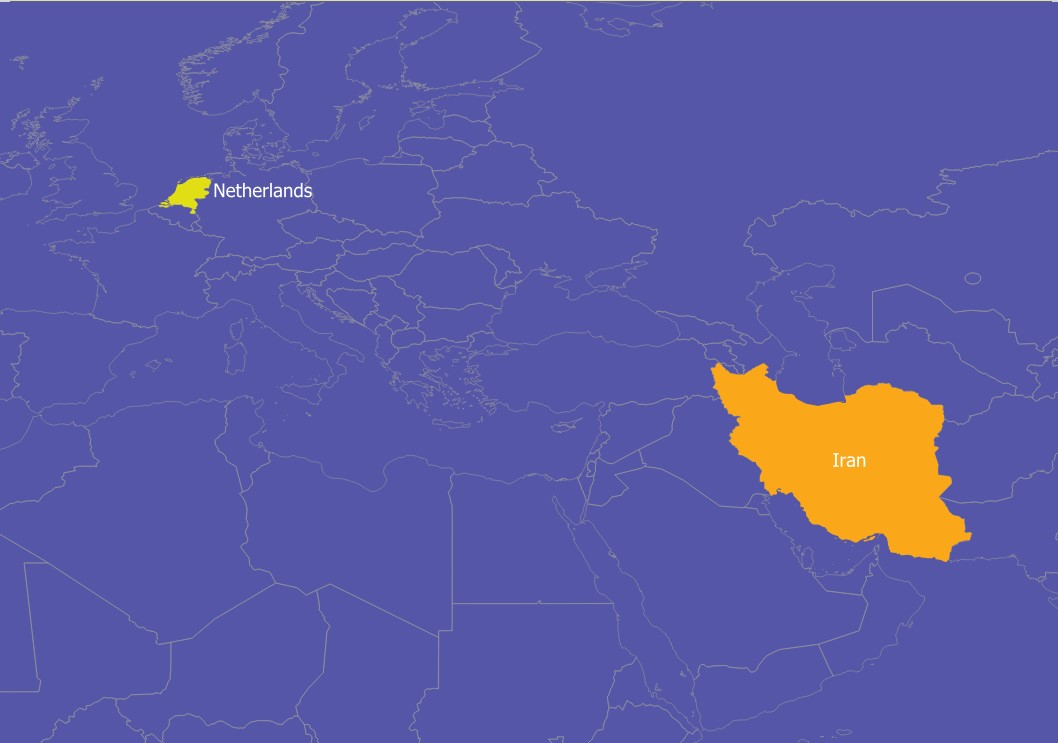
\includegraphics[width=4.69792in,height=\textheight,keepaspectratio]{images/map_world_iran.jpg}

}

\caption{\emph{Figure 1. Iran and the Netherlands in the world}}

\end{figure}%

\begin{figure}[H]

{\centering 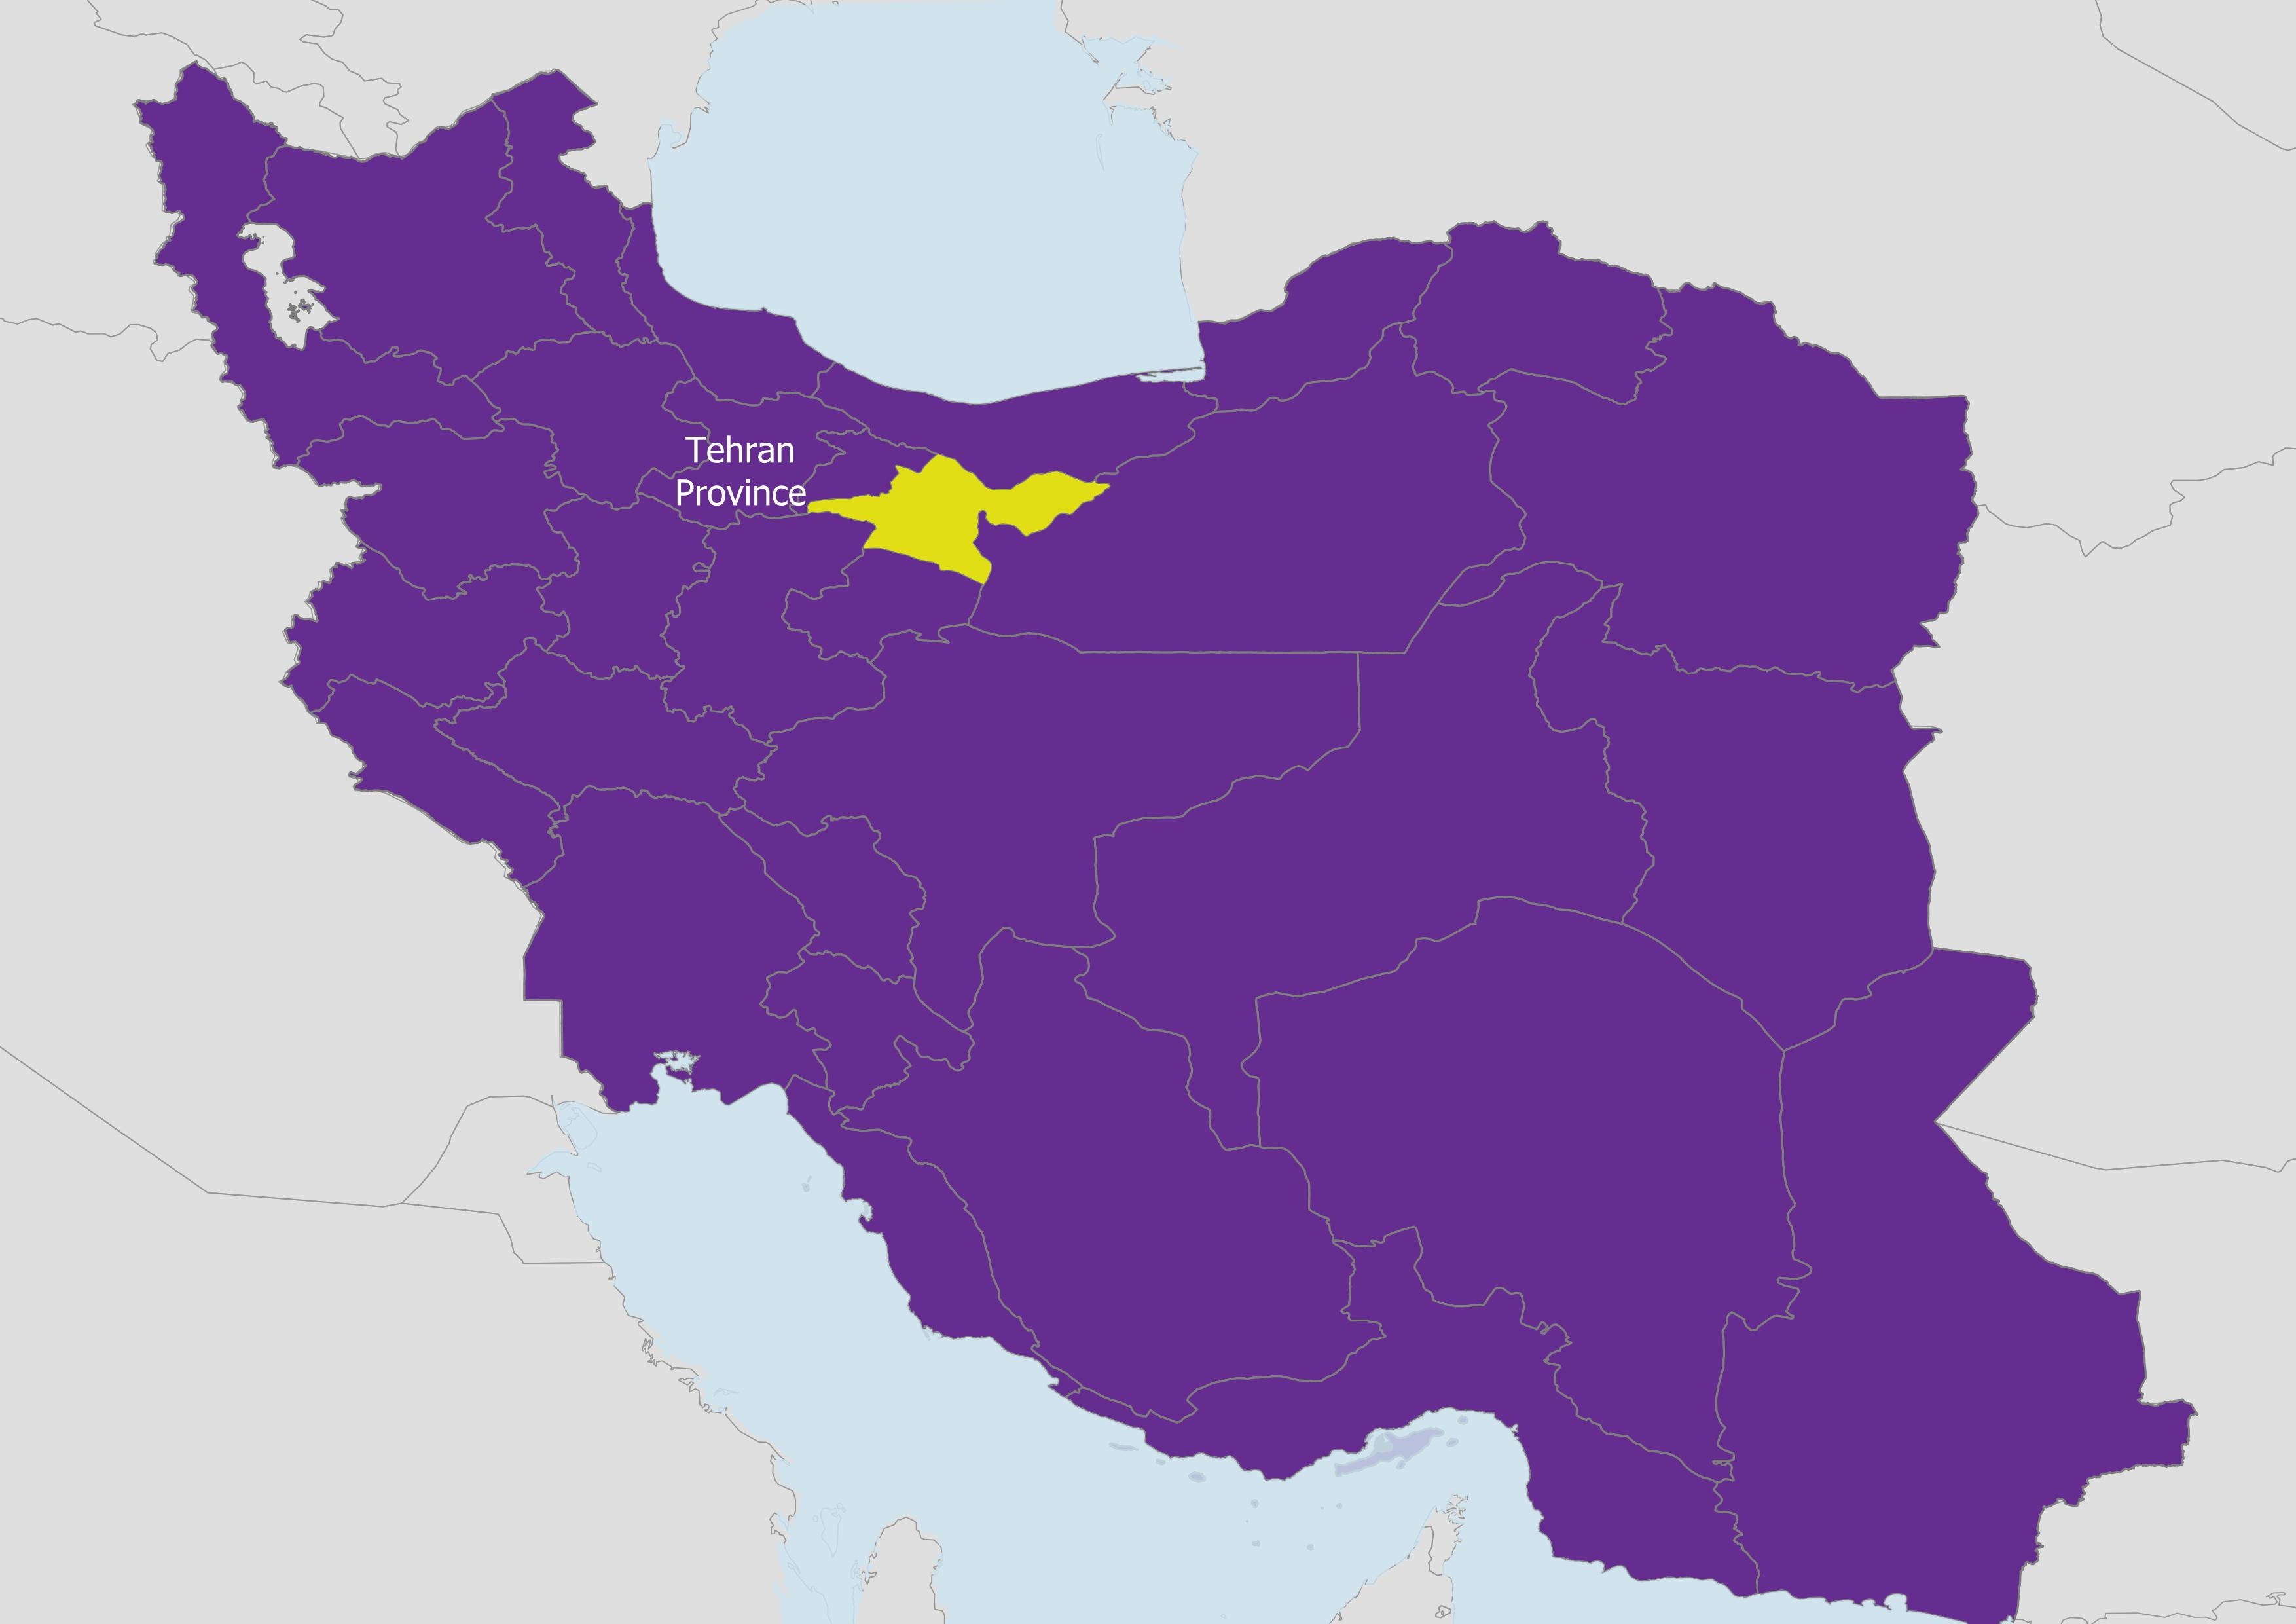
\includegraphics[width=4.66667in,height=\textheight,keepaspectratio]{images/map_Iran.jpeg}

}

\caption{\emph{Figure 2. Tehran Province in Iran}}

\end{figure}%

\begin{figure}[H]

{\centering 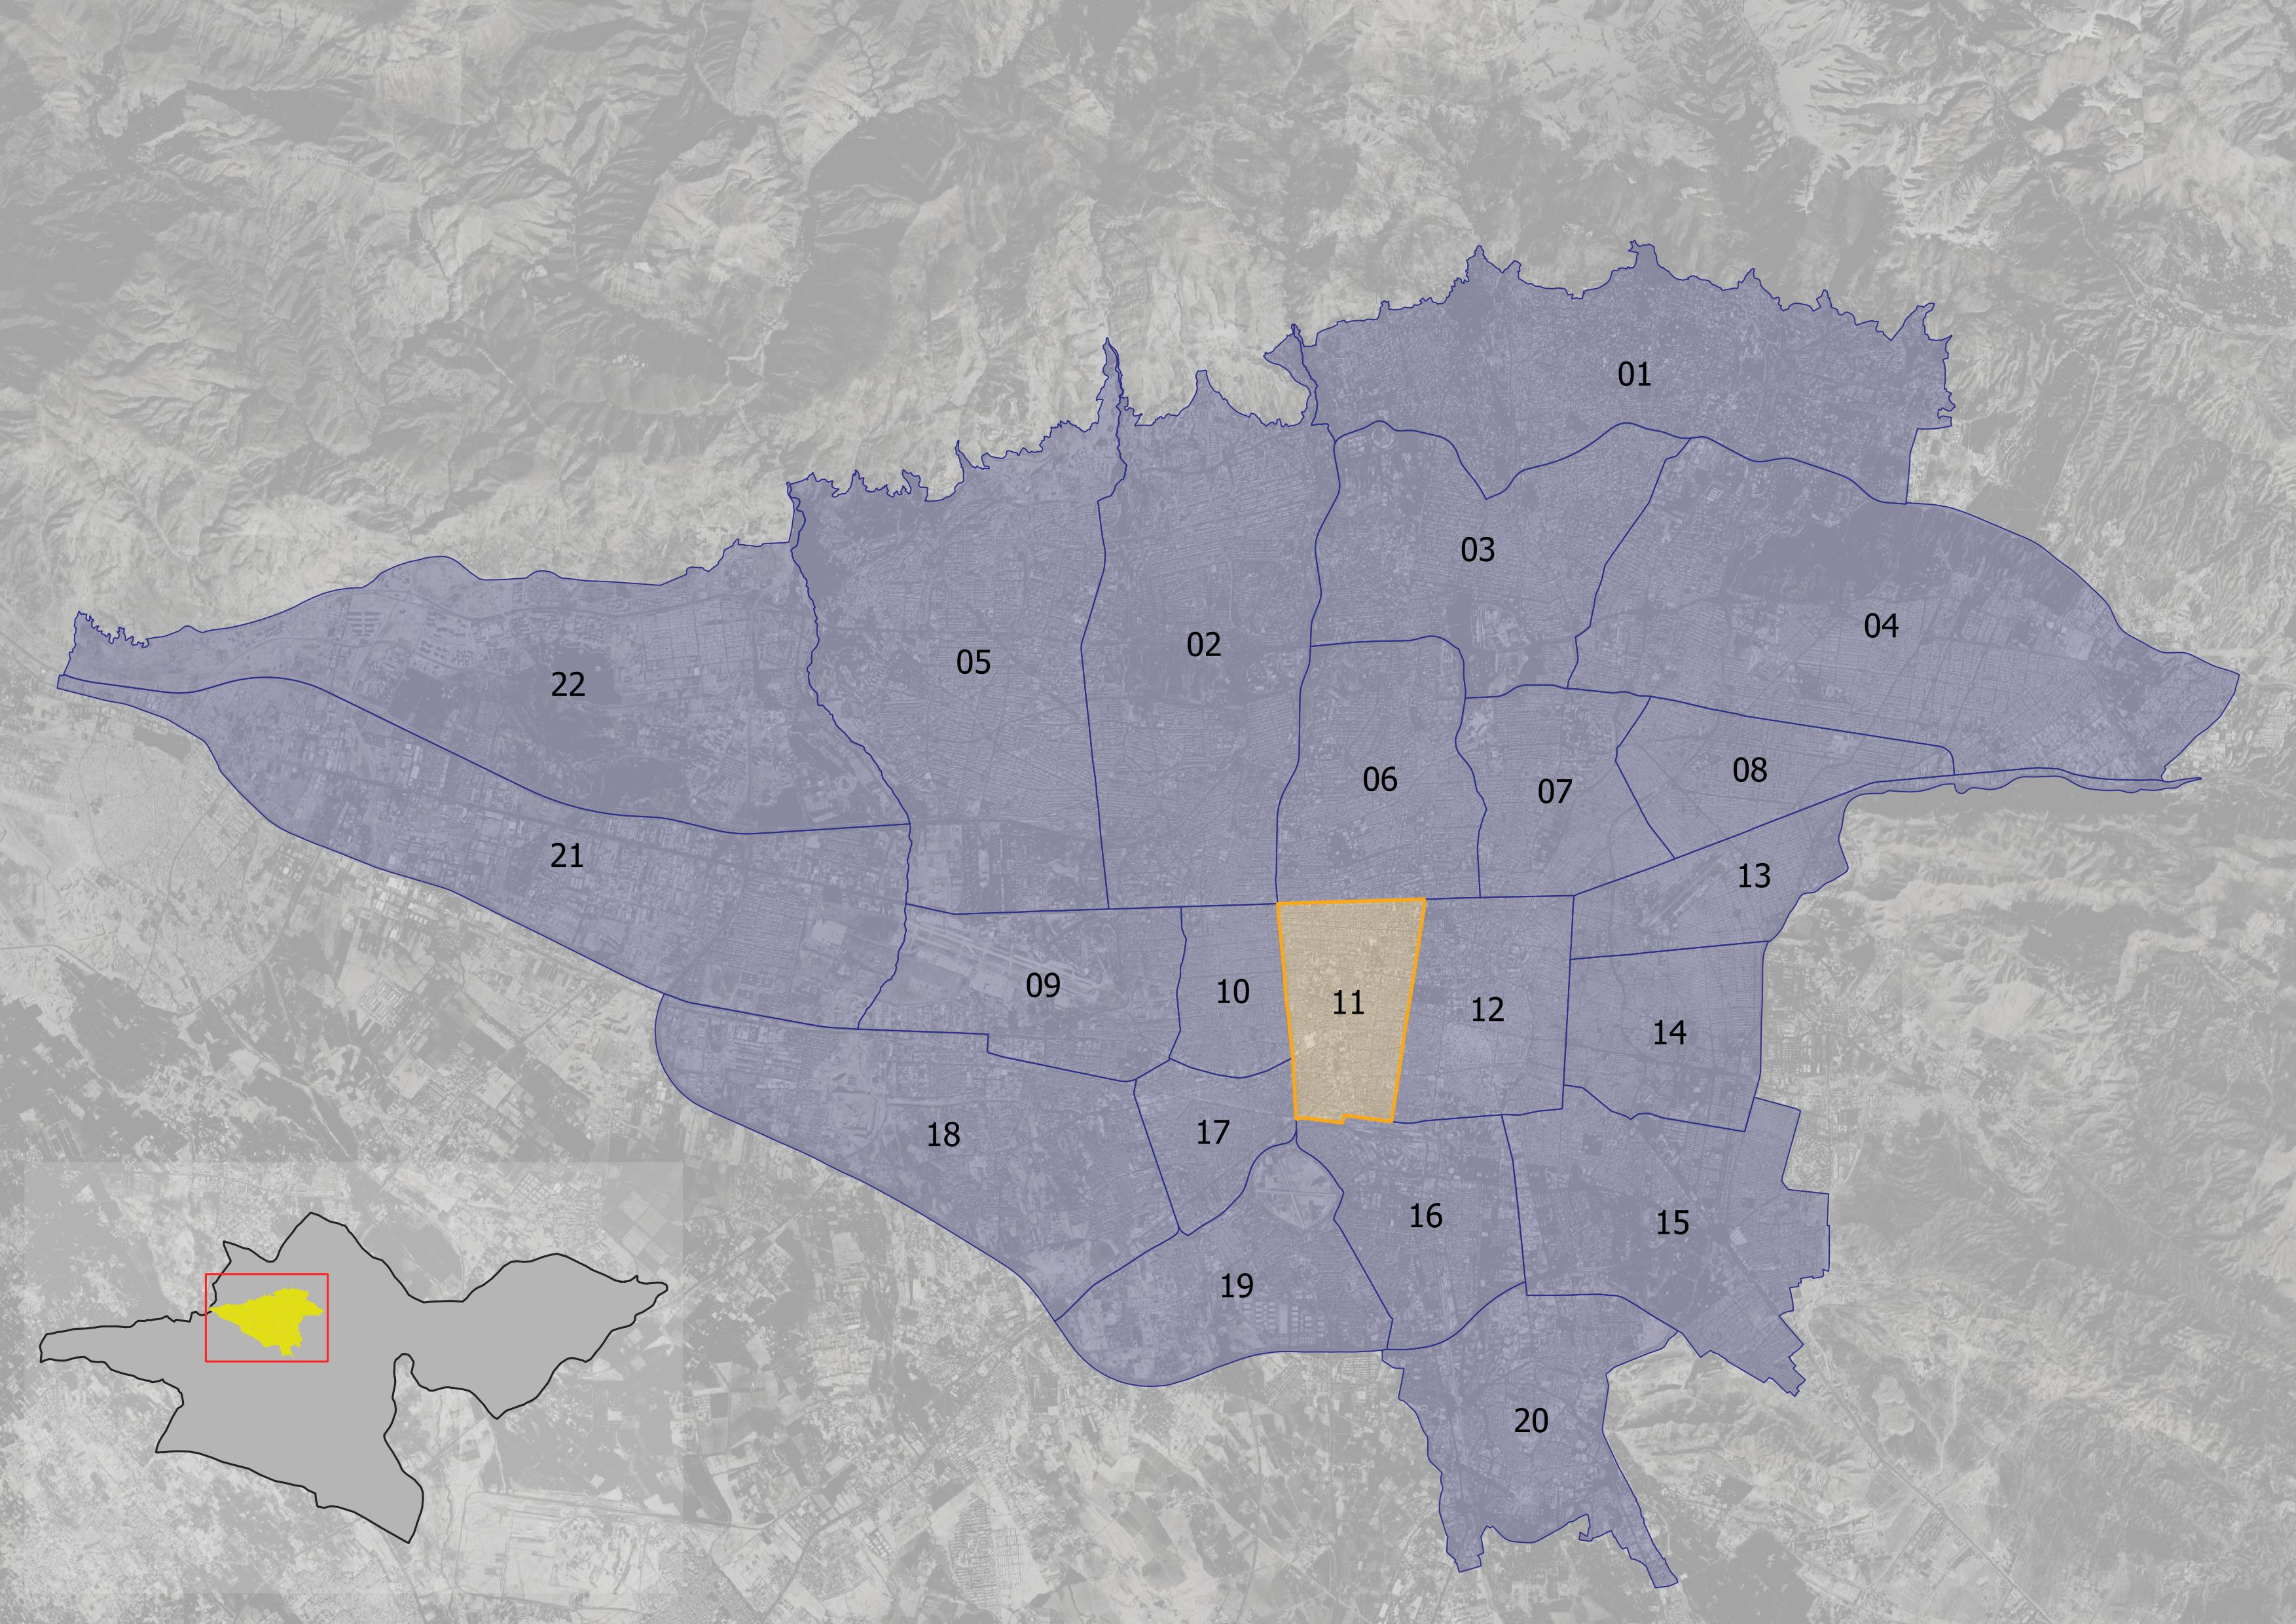
\includegraphics[width=4.64583in,height=\textheight,keepaspectratio]{images/Tehran_districts_2.jpeg}

}

\caption{\emph{Figure 3. Tehran's districts}}

\end{figure}%

In countries like Iran, despite following the theories and works of
citizen engagement in academia, the practice is far behind this mindset.
Many urban development projects are implemented with a top-down
approach, regardless of who is responsible. Whether a contractor,
developer, designer, planner, or policy maker, none ever approached the
public for their opinions on an urban project. There are minimal
practices that tried to include citizens within their work by running
surveys or interviews. Nevertheless, the number of participants has
barely met the needs of the affected population, which looked more like
manipulation (Arnstein 2019). The planning and design approaches in
countries with less democratic political systems would yield the least
successful public engagement through their processes.

Although active participation has never been easy, tools and platforms
have made the process smoother for both parties. In the digital era,
many citizens have access to online social platforms where they can
usually speak up for themselves, with the chance that their opinions
could be heard nationally and even globally. In such an era, Iran is not
an exception either. Although Iranians have filtered internet access,
they use VPNs to bypass the restrictions and access the free internet,
sharing their opinions, voices, cries, compliments, memories, and other
experiences that are inaccessible on online social networks.

This new accessibility can be considered as a shortcut to democracy.
Sharing news and posts about urban spaces is an ongoing phenomenon that
goes beyond a single media post with a caption. It can be seen as
acknowledging a new space, or, conversely, as downgrading a new
intervention in the city. The background of a city can now be traced
through online platforms run by individuals who captured it over time.
This doesn't end with the past of urban spaces, but also with how urban
spaces change in real time, which would have its own responses. How
citizens react to an urban project is evident on social media, and how
they perceive the transformed urban space is evident as well. The urban
space is not just a physical or mental entity; it's also digital.

This study aims to examine how citizens' lived experiences shared on
social media form urban digital memories. Digital memory creates new
concepts on top of the notion of the right to the city, which can be
called the right to the memory. \textbf{The project focuses on how the
right to the memory can serve as a significant tool for validating urban
interventions in spatial features through a digital public engagement
and participation perspective.}

\begin{figure}[H]

{\centering \pandocbounded{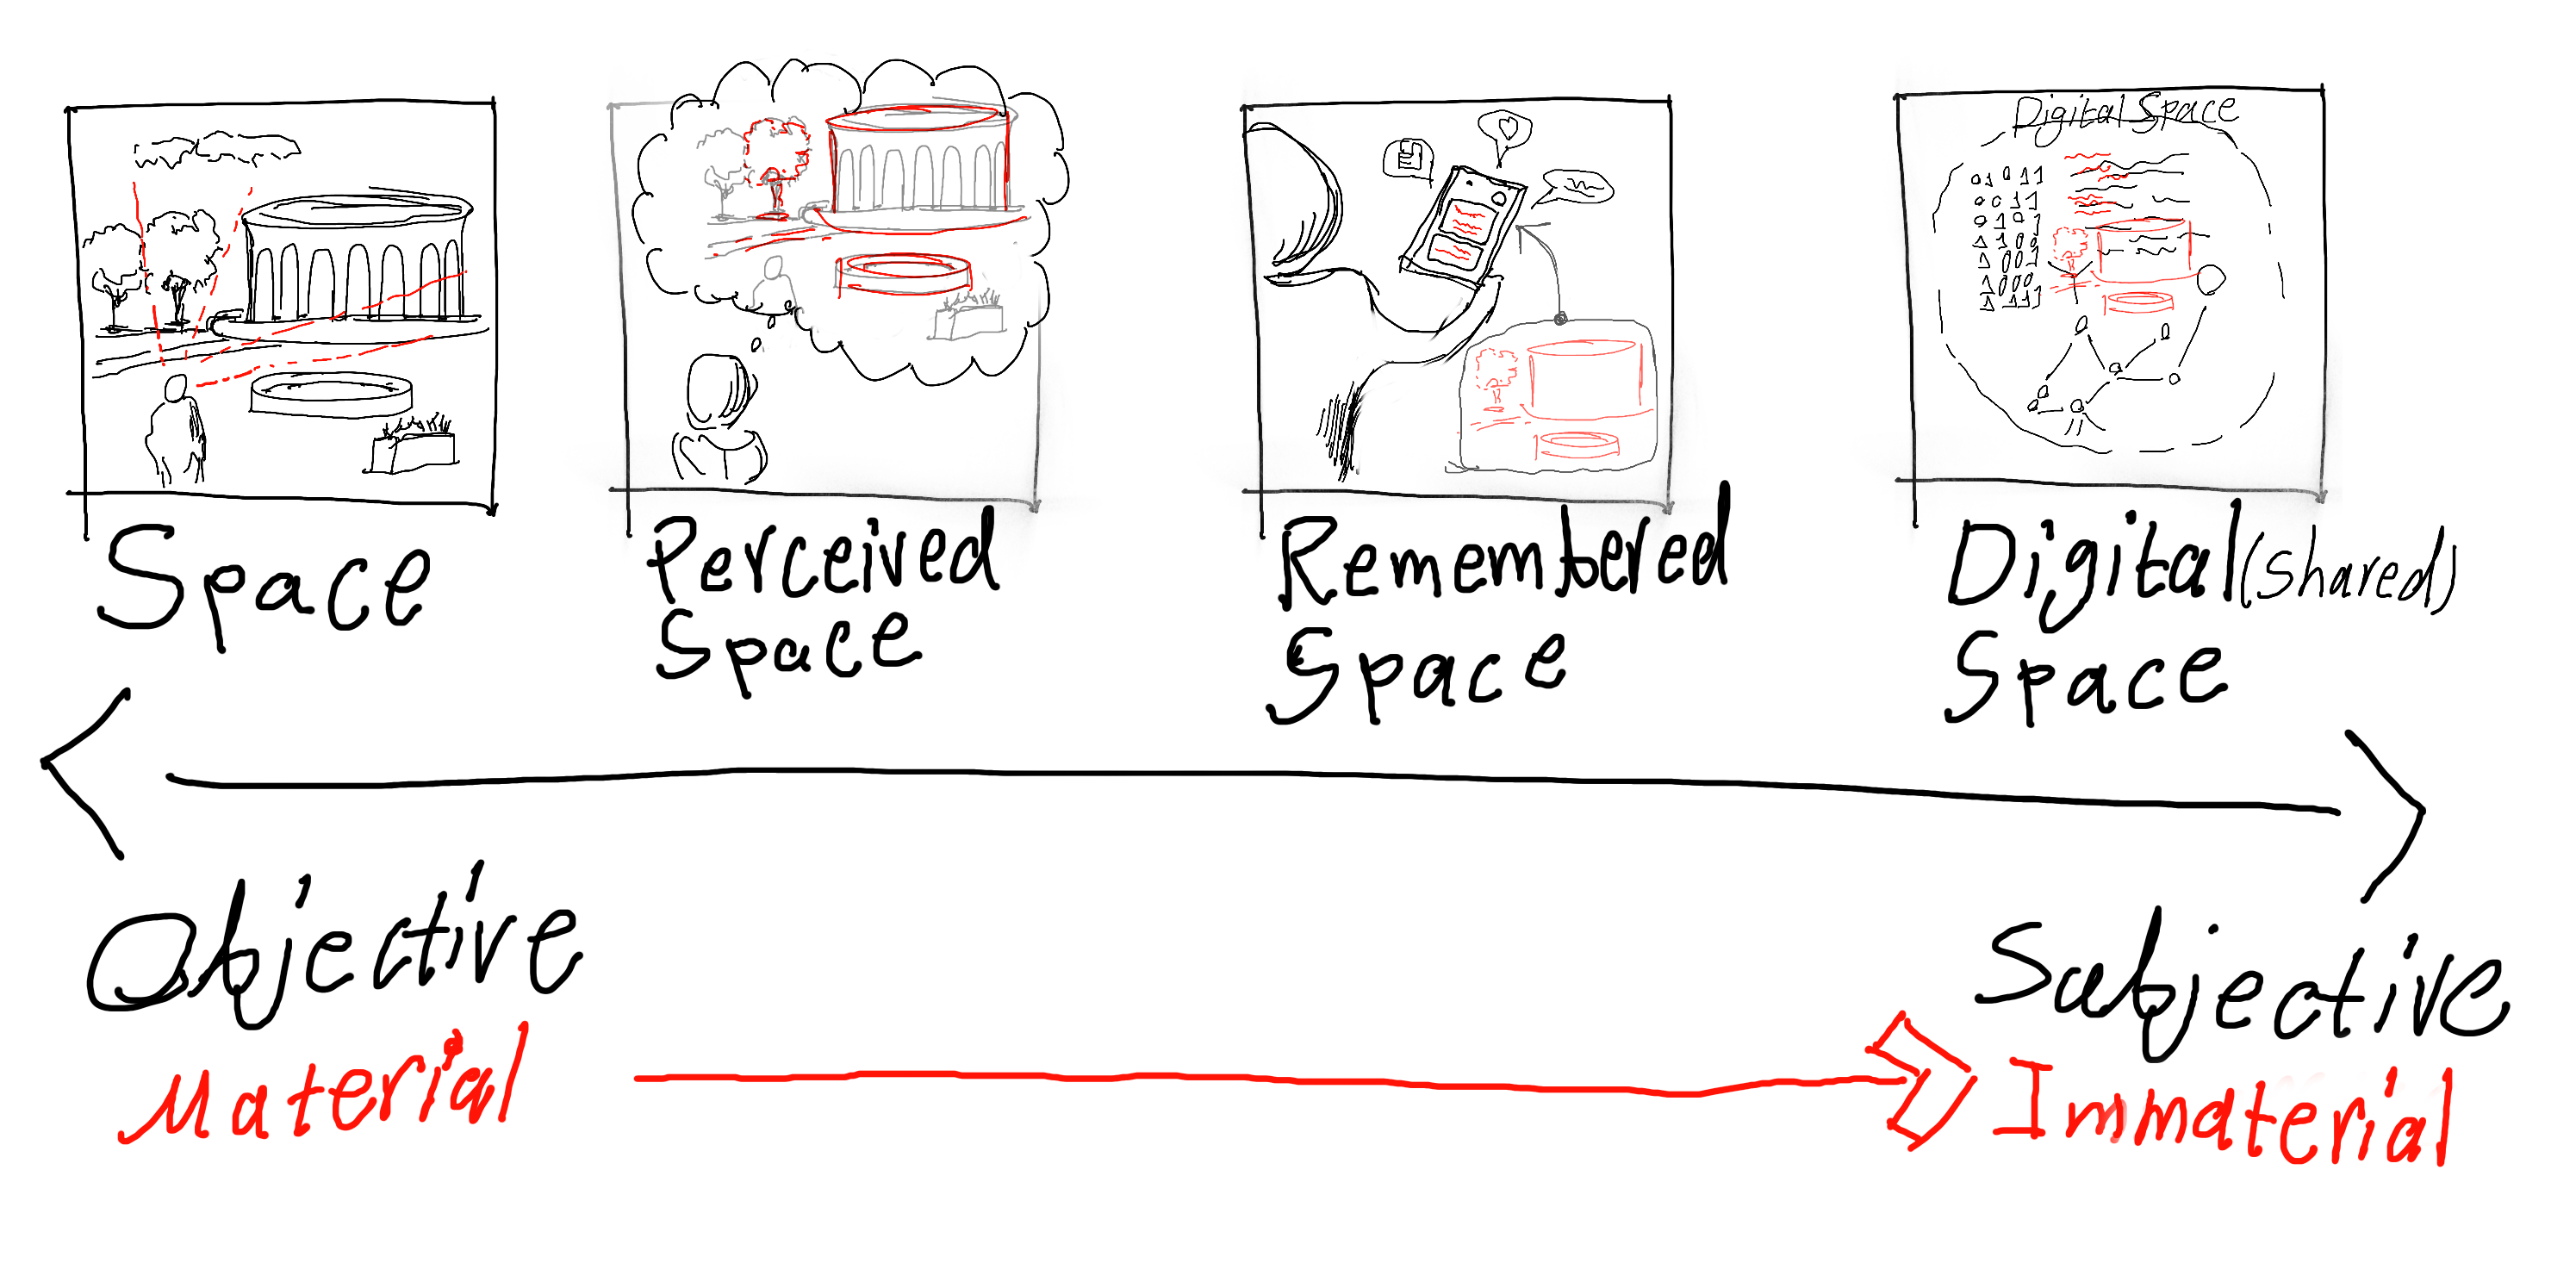
\includegraphics[keepaspectratio]{images/-space-.png}}

}

\caption{\emph{The Urban Digital Memory}}

\end{figure}%

\subsection{City Theater of Tehran (Teatré Shahr-e
Tehran)}\label{city-theater-of-tehran-teatruxe9-shahr-e-tehran}

One of the public squares that has always been the site of intense
tension between its users and those who want to change it is City
Theater\footnote{Teatré Shahr in Persian {[}Translated by the author{]}}
Square\footnote{The square holds the city theater building within its
  space, which could be considered a semi-open public space in Tehran,
  with all of the activities and events that take place downtown.}. As
can be seen in (Fig. 4), the square is in the intersection of Vali'asr
and Enghelab streets, which are the longest NS / EW armatures of Tehran.
The space is located in District 11 of Tehran's municipality.

\begin{figure}[H]

{\centering 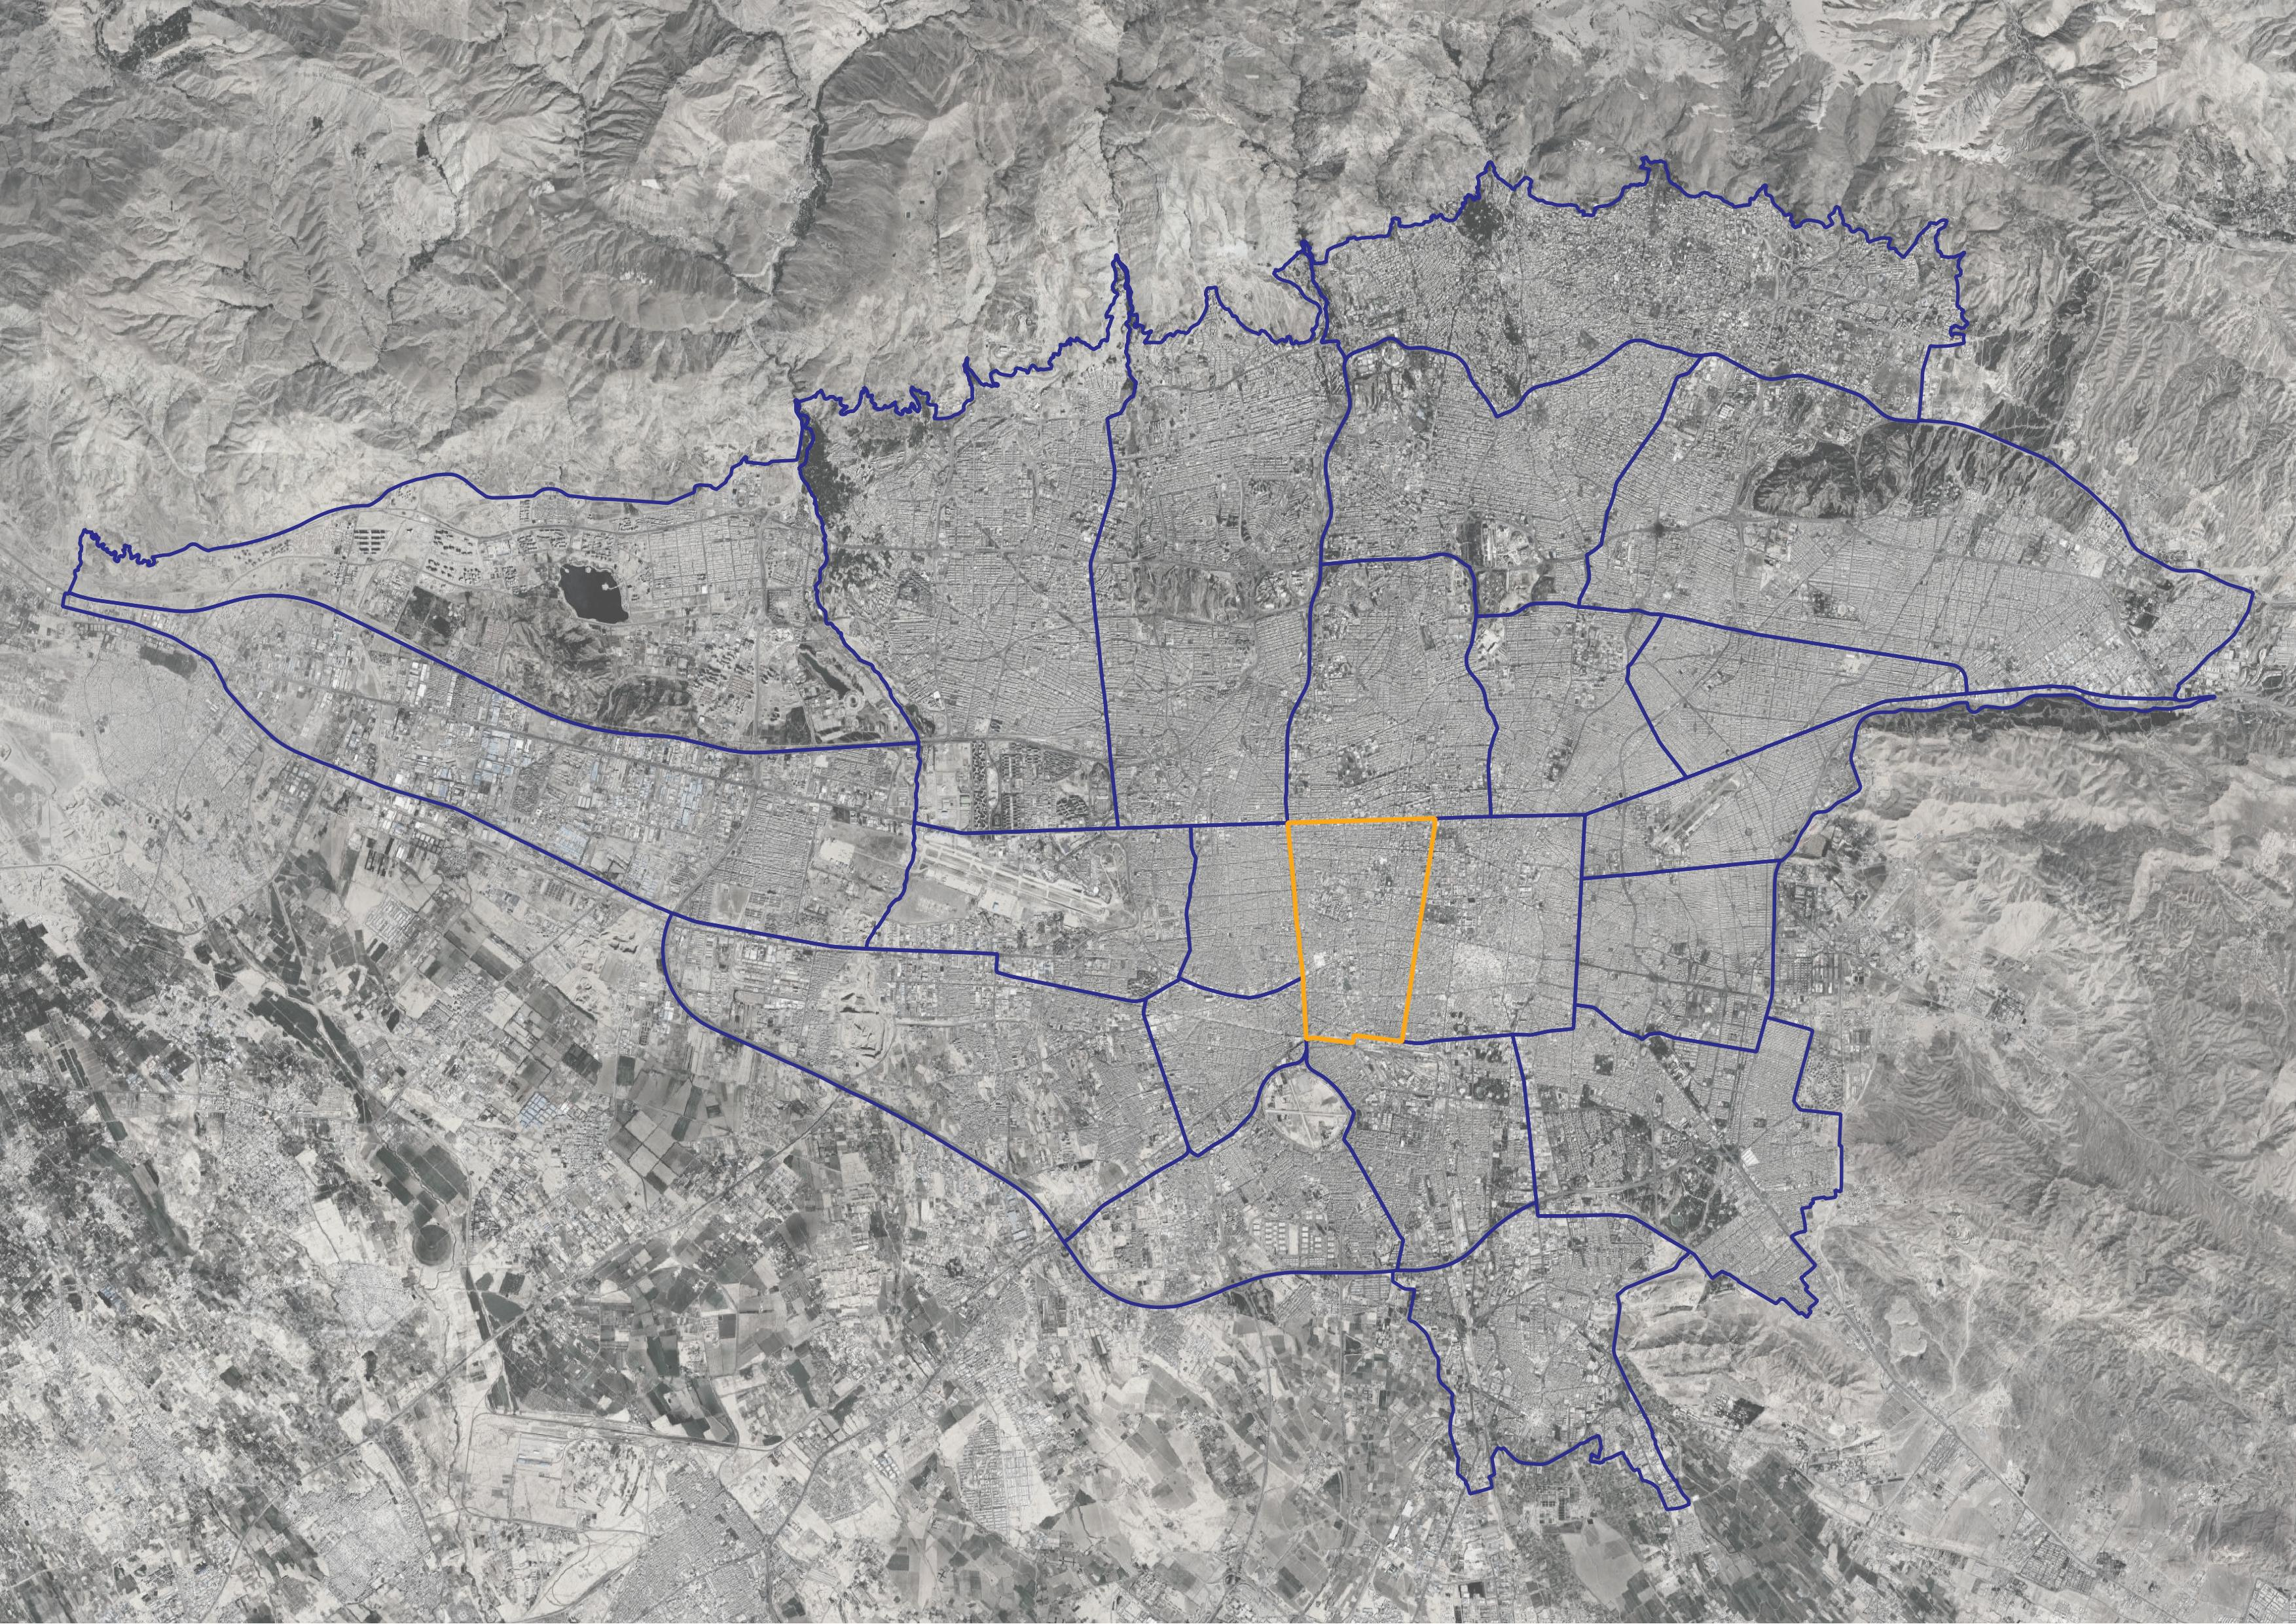
\includegraphics[width=5.33333in,height=\textheight,keepaspectratio]{images/city theater_2.jpeg}

}

\caption{\emph{Figure 4. City Theater Plaza's location in Tehran\\
Source: Google Map Satellite, 2026.}}

\end{figure}%

The City Theater Square holds one of the oldest theaters in Tehran,
dating back to the 1970s. The City Theater of Tehran building was built
as an art and cultural complex. City Theater was not only a venue but
also a taste of contemporary design inspired by Iranian
architecture(wikipedia 2026; Mohit 2026). The presence of the building
and its surroundings formed a public space, as the complex was ready for
productive use.

\begin{figure}[H]

{\centering 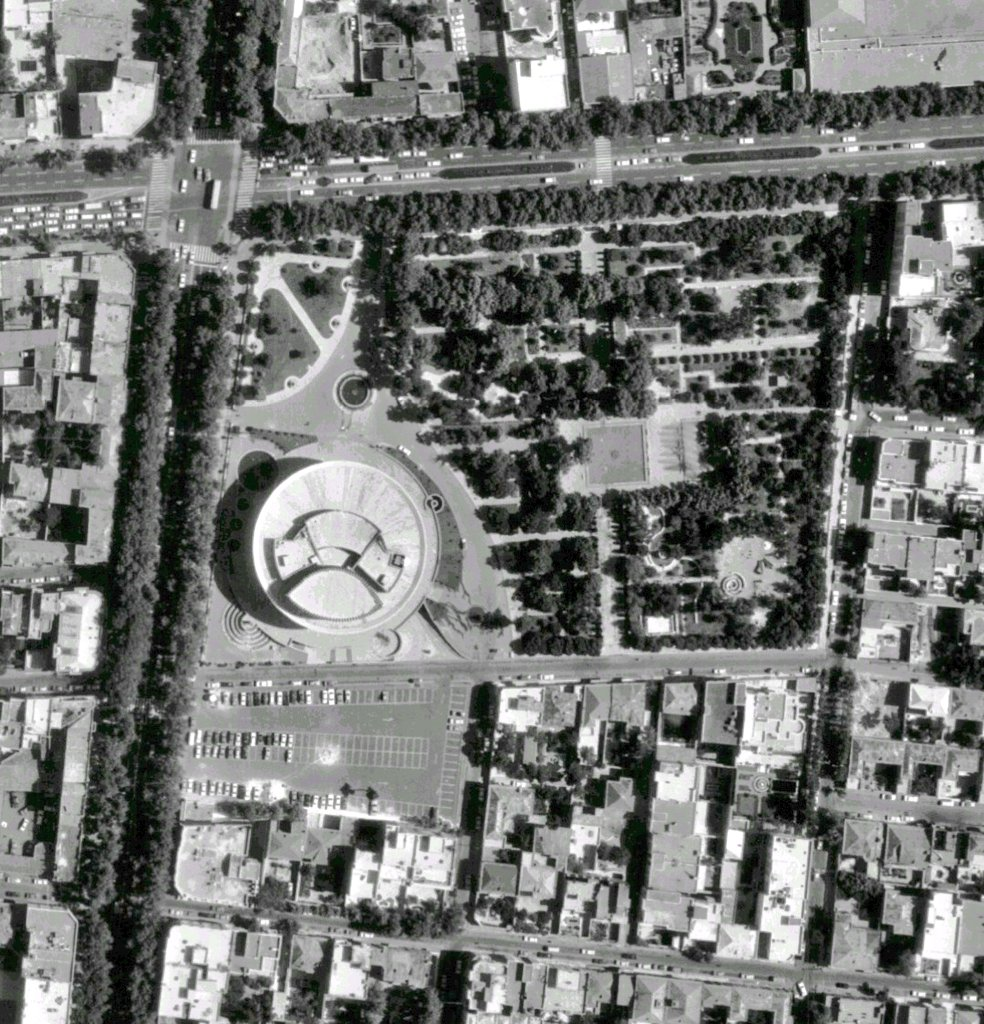
\includegraphics[width=4.83333in,height=\textheight,keepaspectratio]{images/20260121_183415.jpg}

}

\caption{\emph{Figure 5.} Aerial photo of City Theater Plaza and
Daneshjoo Park \emph{in 1975.\\
Source:
\href{https://x.com/i/status/1741505739120590987}{Ehsanrostamipour,
2023.}}}

\end{figure}%

The City Theater used to look like a complex with its specific plaza in
front of the theater's main building entrance (Fig 5). The current
Daneshjoo park, neighboring the Theater's building, was larger than it
is now, covering the northern side of the City Theater that touches
Enghelab Street. Based on the documentation of a user who shared the
aerial image on X (formerly Twitter), the spatial layout in the image is
the earliest and most original spatial intervention in this space.

\begin{figure}[H]

{\centering 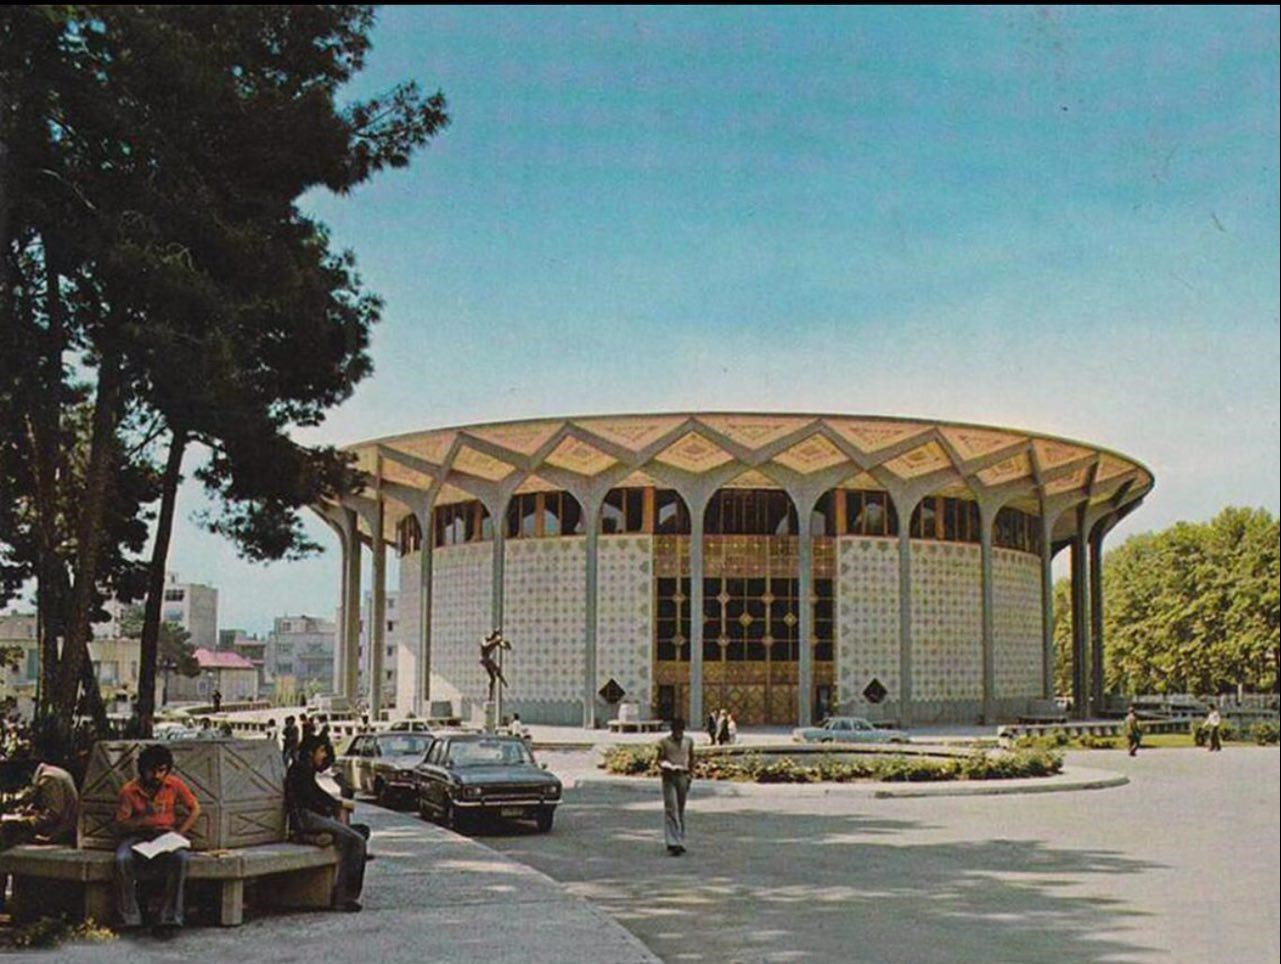
\includegraphics[width=5.32292in,height=\textheight,keepaspectratio]{images/City_Theater_of_Tehran_-_1971.jpg}

}

\caption{\emph{Figure 6. City Theater Building of Tehran in 1971.\\
Source: Wikimedia, 2026.\\
}}

\end{figure}%

\begin{figure}[H]

{\centering 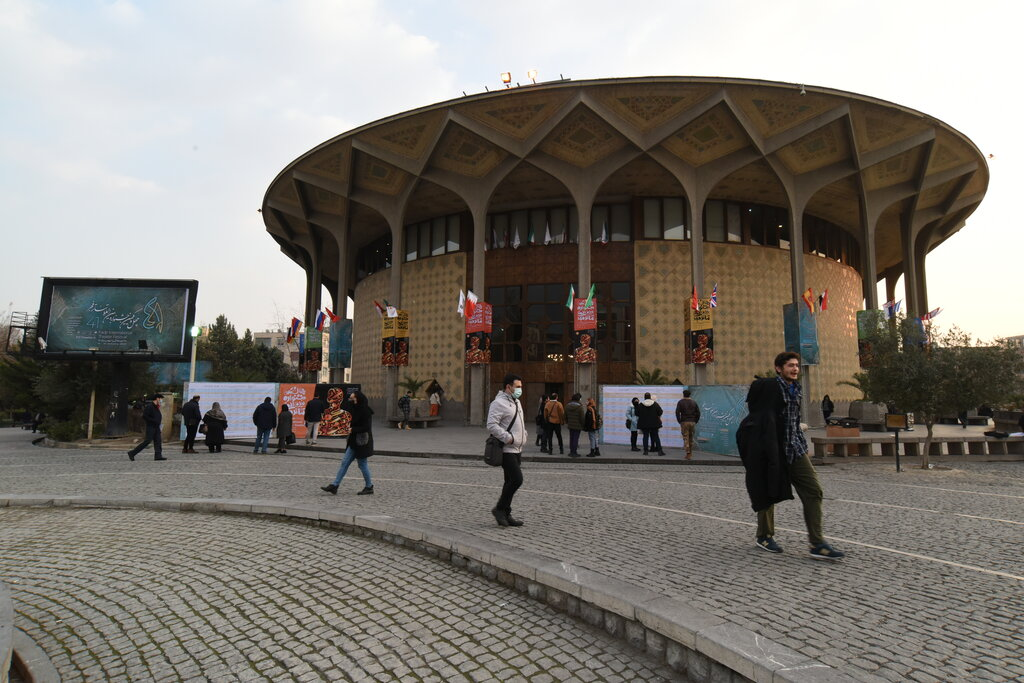
\includegraphics[width=5.29167in,height=\textheight,keepaspectratio]{images/4811609.jpg}

}

\caption{\emph{Figure 7. City Theater's building and plaza.\\
Source: Hamshahri Online, 2024.}}

\end{figure}%

As shown in Figs. 6 \& 7, the building and the plaza surrounding it have
undergone many transformations, including changes in spatial
composition, accessibility, mobility, vegetation, and urban furniture.
City Theater Square has always been a central point of the daily urban
life of Tehran. Moreover, the square has been the ground of various
social and political events since its establishment.

\begin{figure}[H]

{\centering 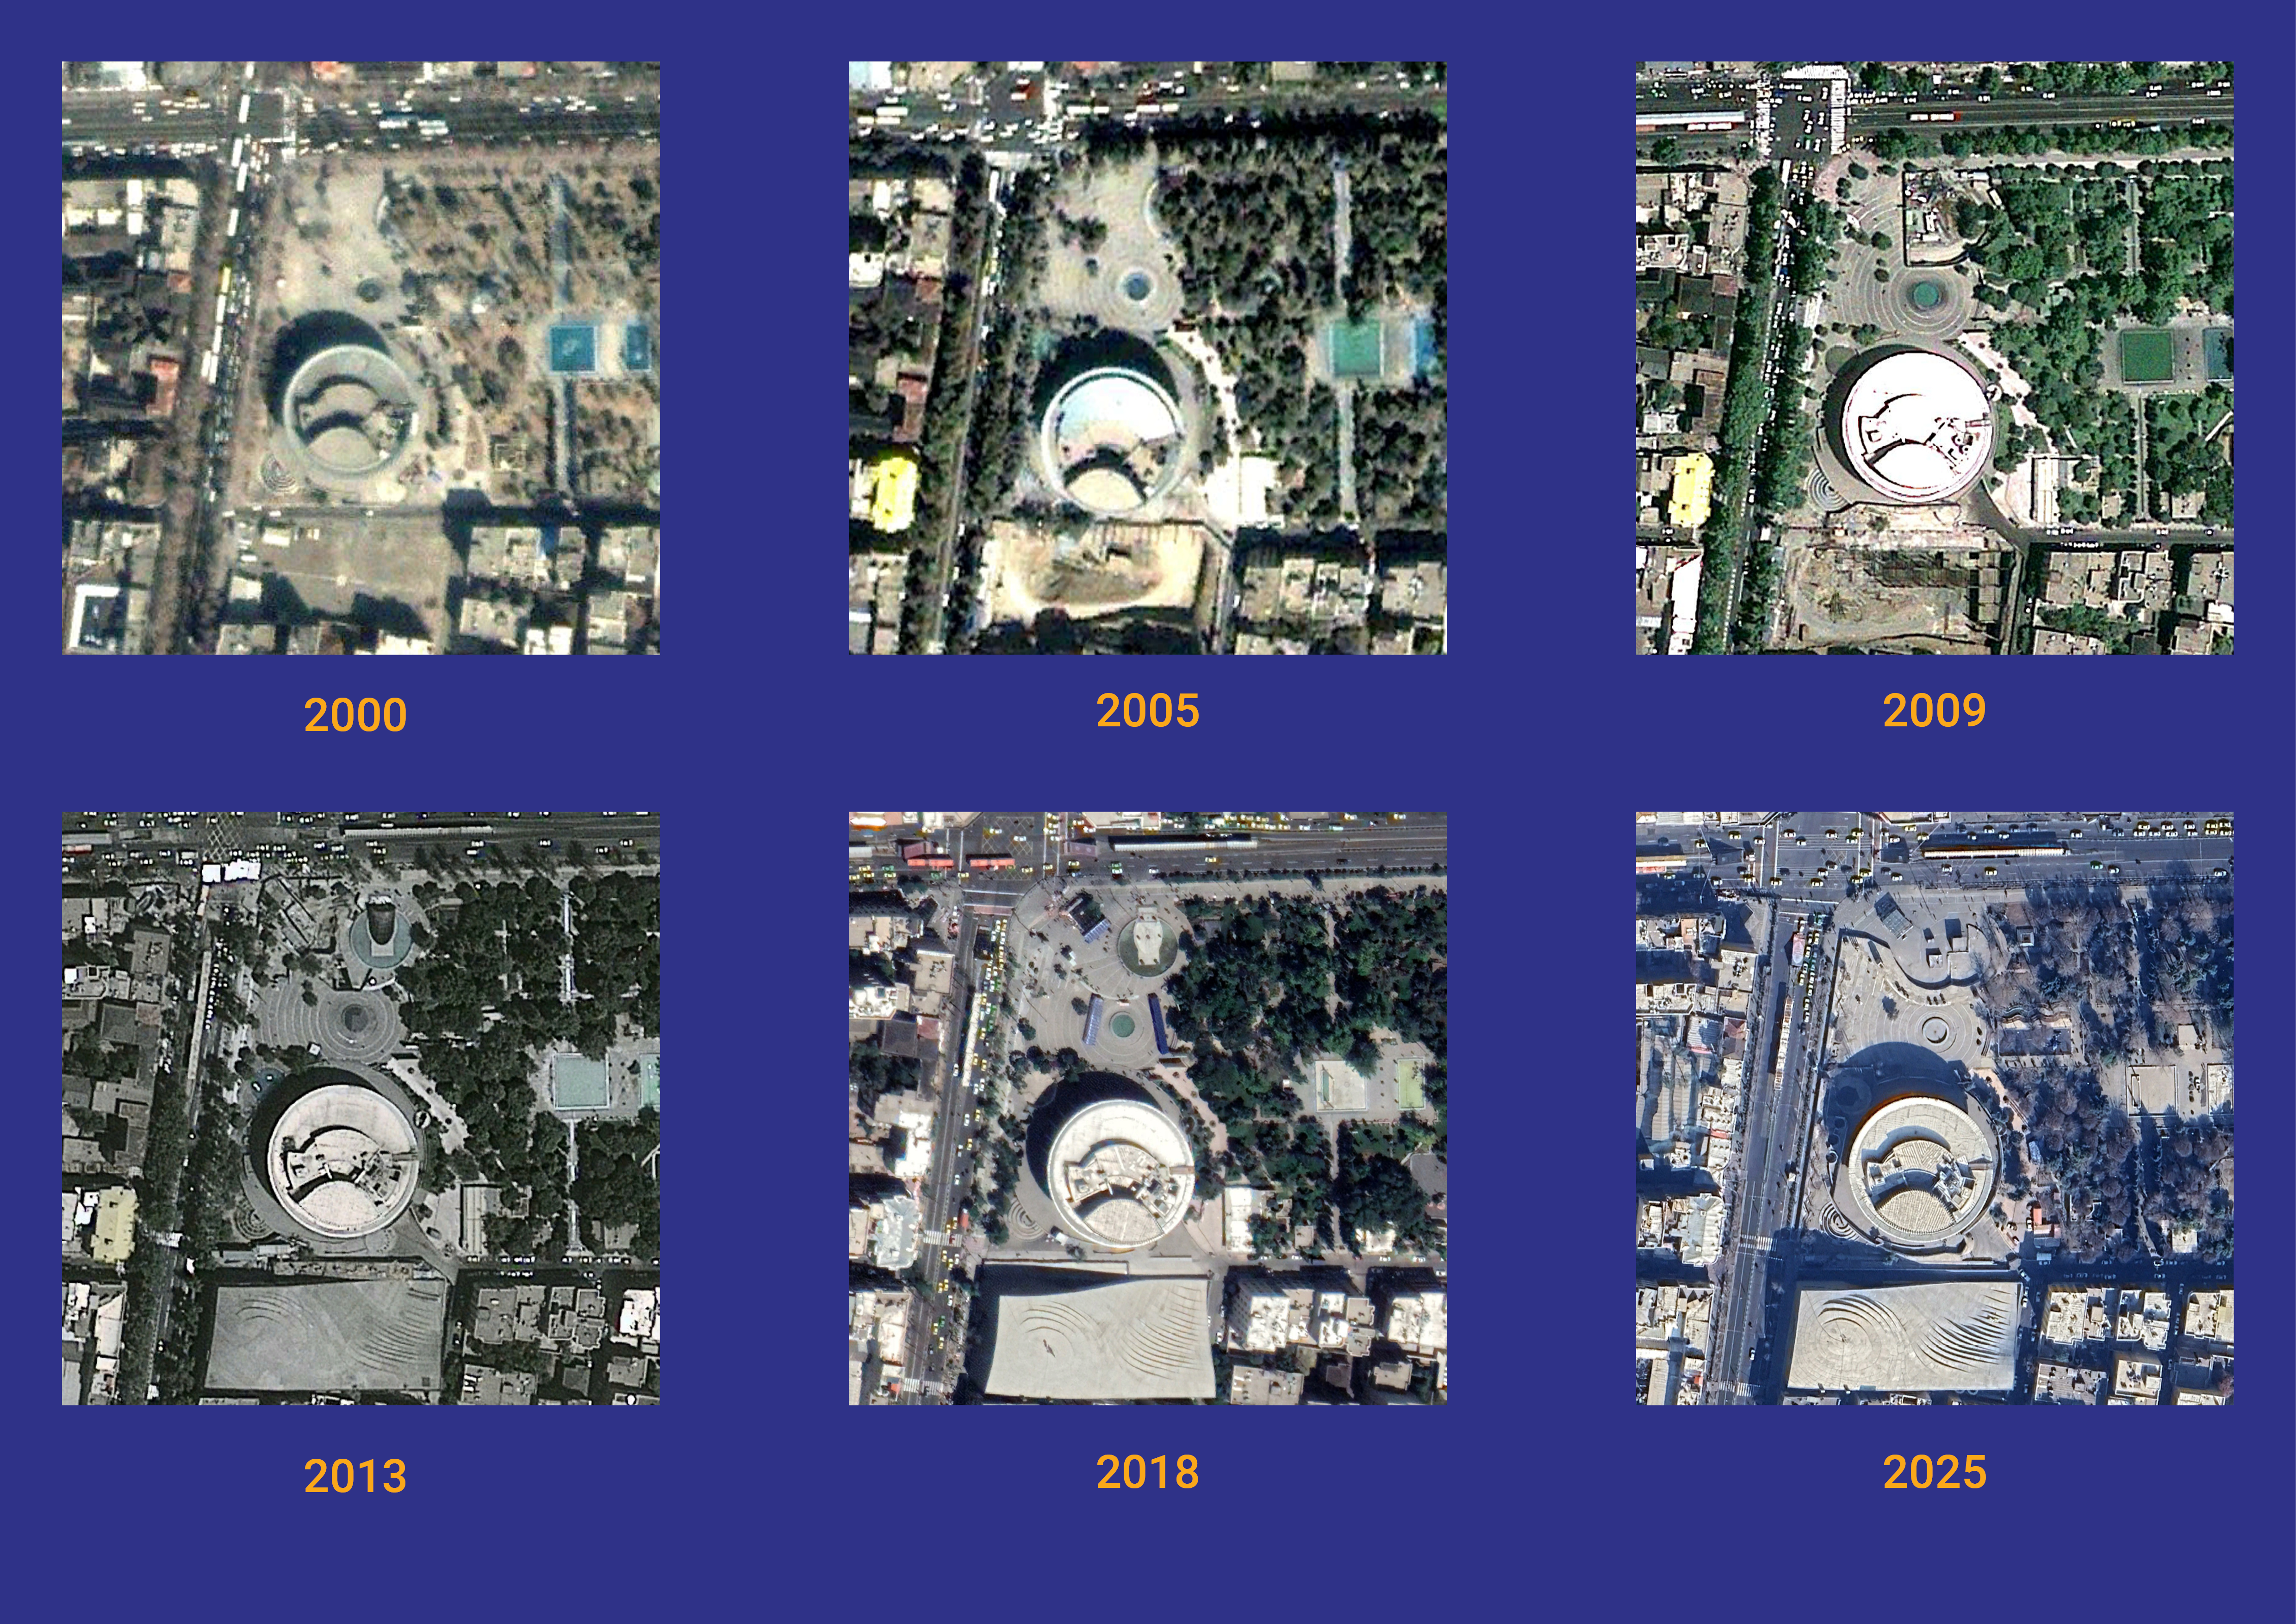
\includegraphics[width=5.5625in,height=\textheight,keepaspectratio]{images/imageries_blue.png}

}

\caption{\emph{Figure 8. City Theater Square transformations between
2000 and 2025.\\
Source: Google Earth Engine, 2026.}}

\end{figure}%

The City Theater plaza has undergone several transformations over the
decades (Fig. 8). Various small- and medium-scale interventions have
been implemented within its space, from removing statues to constructing
the underground path, pedestrian access, and the metro station entrance.
Some of these transformations are traceable through Google Earth's
satellite imagery. However, the satellite images have been captured
since the 2000s. Yetthey make significant spatial interventions, whether
inside the plaza or outside, around the square and the main streets of
Tehran.

\newpage{}

\section{Problem Statement}\label{problem-statement}

There are urban spaces, specifically, public spaces that hold a large
pool of collective and individual memories within them, either tragic,
joyful, or revolutionary (Solnit 2009). City Theater's Square\footnote{Teatré
  Shahr in Persian {[}translated by the author{]}} is not an exception.
However, the public apparently has no right or authority over the space
and its memories as common property. Some spaces are manipulated,
transformed, or even demolished by governments, driven by economic or
political interests(Paccoud 2016; Solnit 2001). An example could be the
Haussmannian boulevards, which demolished existing urban streets,
creating wide, long boulevards lined with luxury retail shops and police
to oppress any citizen opposition in the most dominant way
possible(Harvey 2006). All of the valuable memories and the space known
to the public were lost in the blink of an eye (Solnit 2001). The
citizens don't have any agency over the space or its corresponding
memory to make decisions, or at least to be clearly informed about the
interventions and changes made by the actors on higher ground. Not only
to the actors but also to the decision-makers; this applies as well.
Right to the memory is a metaphor of collective/individual rights over
space tied to memories that emerge within it. This represents a bond
between the space and its dwellings and visitors, shaped by memories,
emotions, presence, and activities that have shaped each person's lived
experience in that space. Nevertheless, this connection is taken for
granted by the actors, designers, policymakers, and governments holding
the upper hand. Sometimes it's even ignored by them, or it conflicts
with their main interests.

The memory is a valuable lived experience that holds evidence of a
physical space, conceived and perceived by each individual (Shaw and
Graham 2017). The cognitive perception of space, recorded on an open
platform for sharing with others, has been discussed in the literature.
As Solnit (2001) aesthetically showcases the typicality in urban daily
life that may be only engraved in literature, it can emerge in the
digital space as well. Social media can store individuals' most typical
daily routines, written by them, like a diary.

\begin{figure}[H]

{\centering 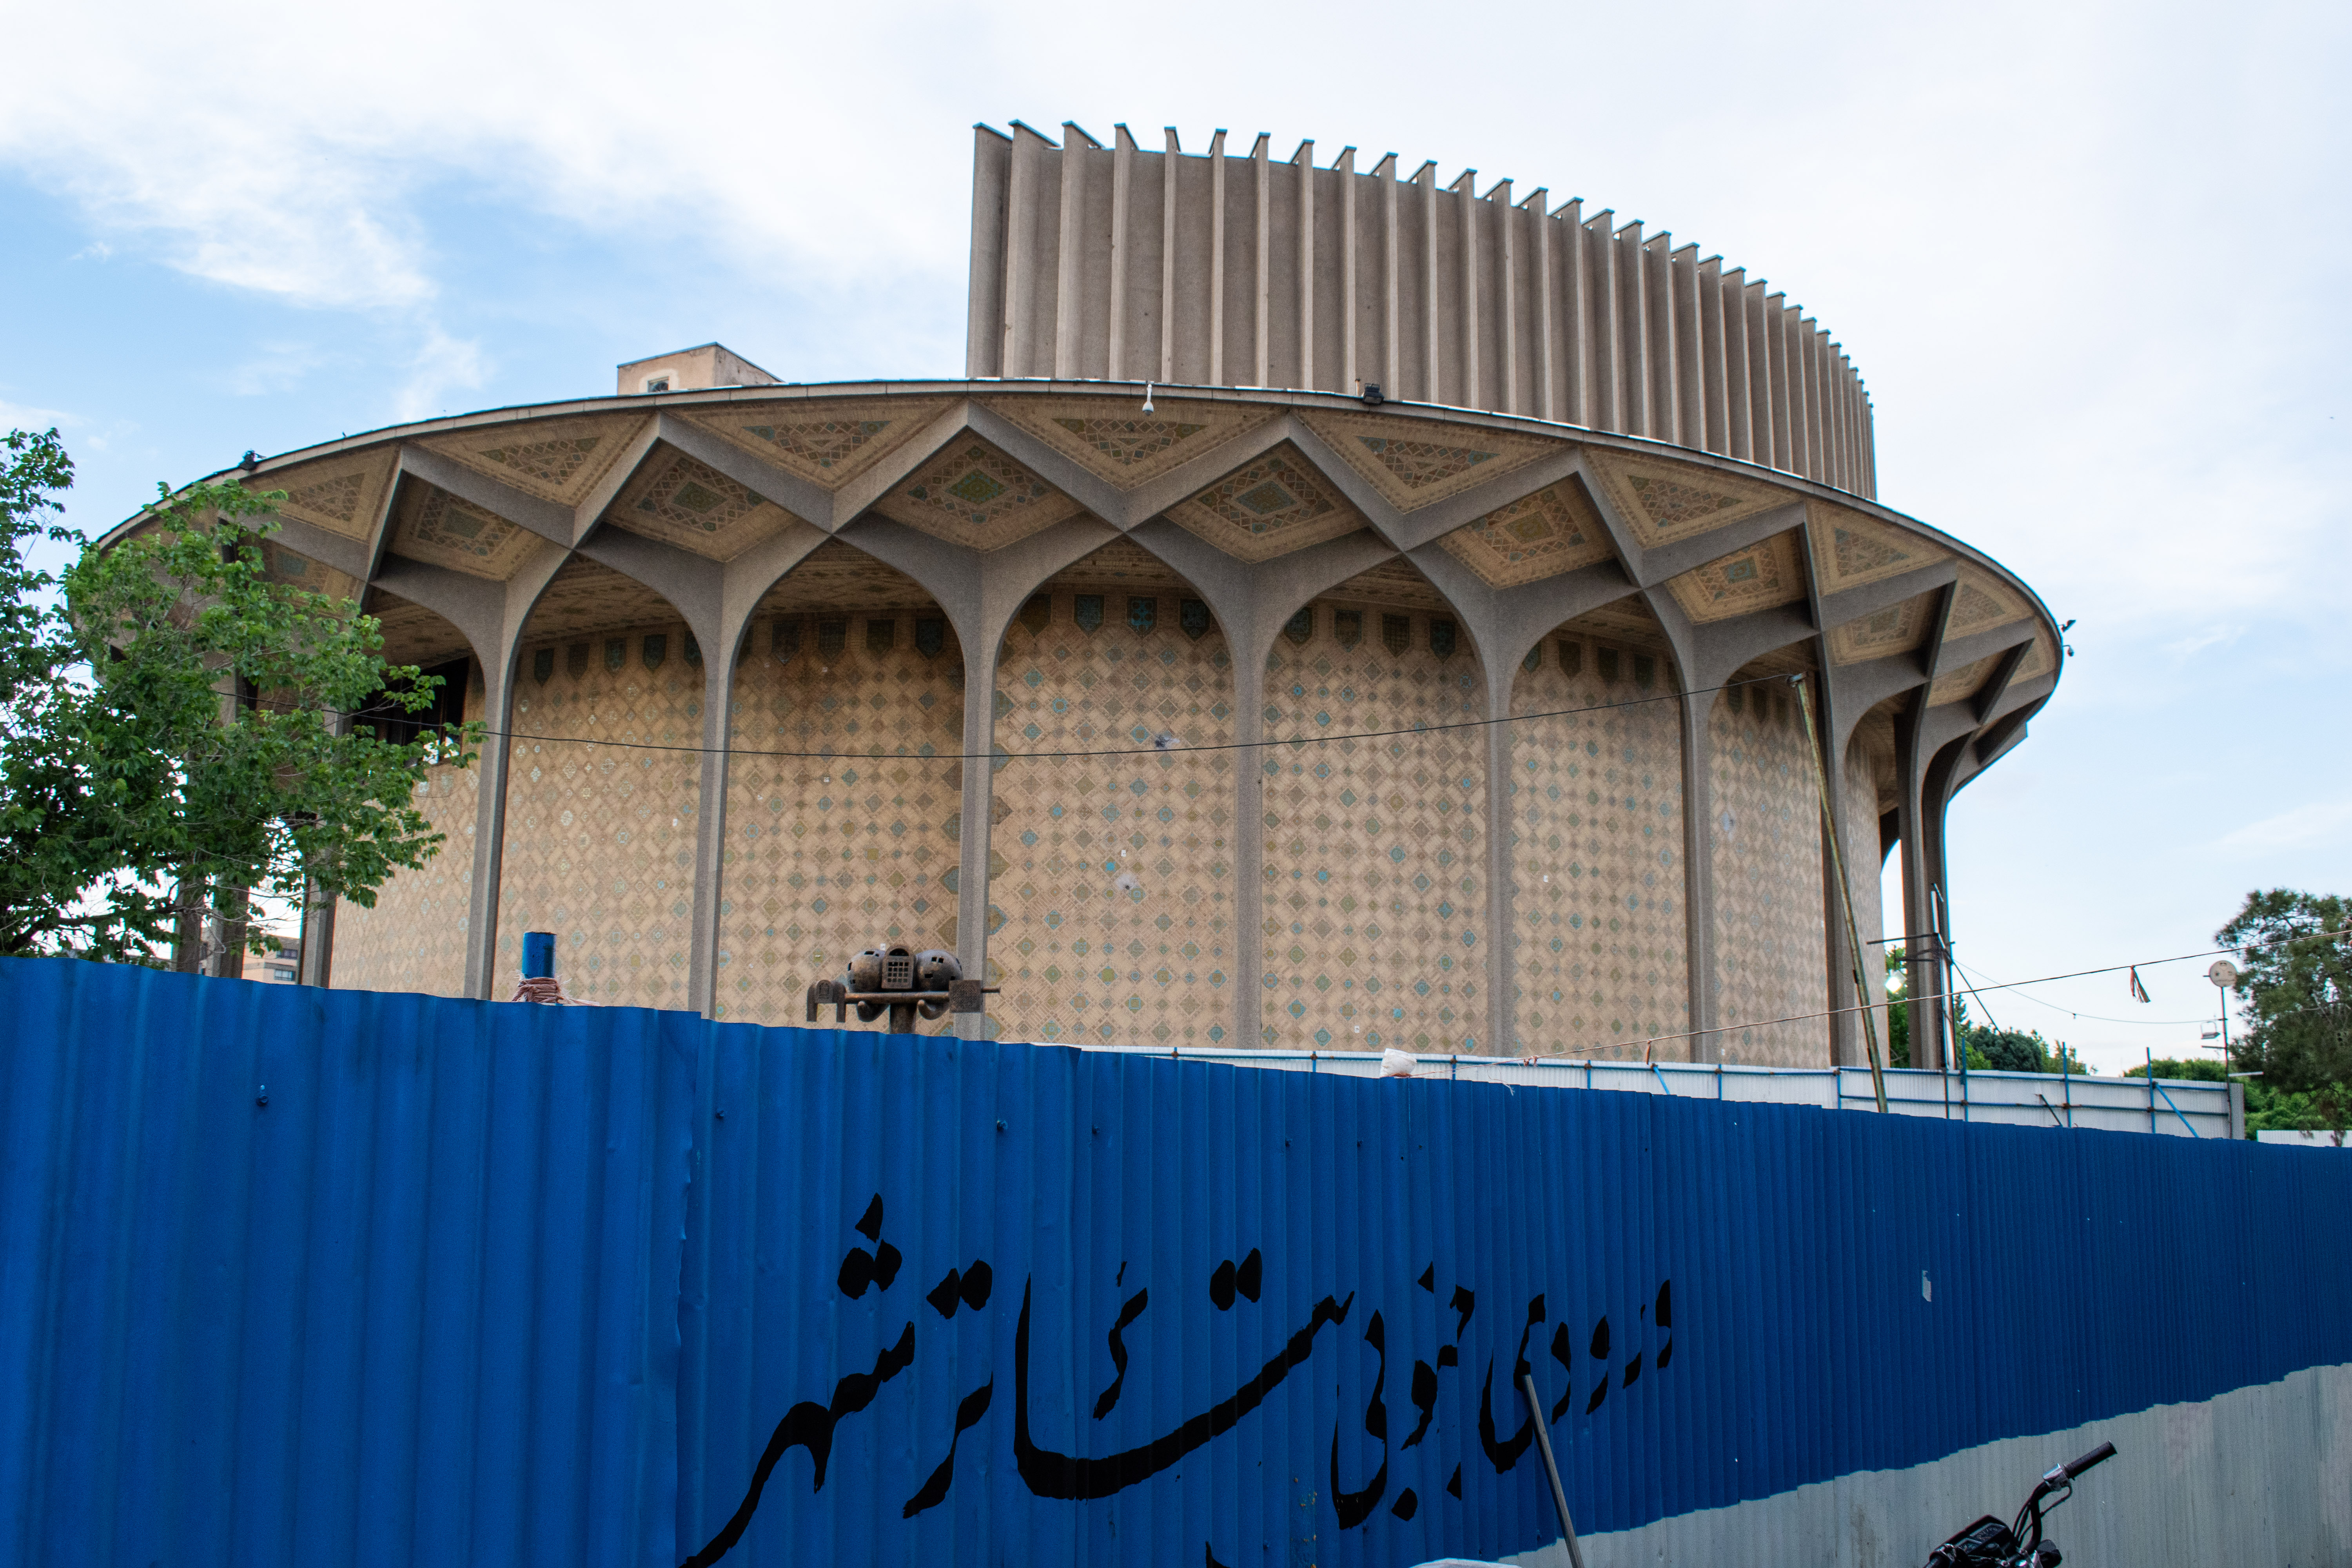
\includegraphics[width=4.47917in,height=\textheight,keepaspectratio]{images/Théâtre_municipal_de_Téhéran_(1)_2024.jpg}

}

\caption{\emph{Figure 9. Fence placement around City Theater for
reconstruction\\
Source: Wikimedia, 2026.}}

\end{figure}%

\begin{figure}[H]

{\centering 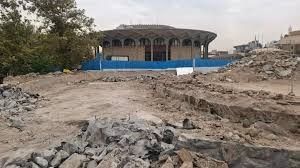
\includegraphics[width=4.26042in,height=\textheight,keepaspectratio]{images/didhonar_2026_corrected.jpeg}

}

\caption{\emph{Figure 10. Demolishing the central space of City
Theater's plaza for reconstruction.\\
Source: Didhonar, 2026.}}

\end{figure}%

The spatial transformation of City Theater's plaza is ongoing. In the
past two years, City Theater faced one of the most drastic
transformations since its establishment. It was when a long fence
divided the adjacent pathways in the southern street and limited
pedestrian access to the square (Fig. 9). A redevelopment project began
to redesign City Theater's plaza. As a matter of fact, no citizen was
aware of this project until its design proposal was shared with the
public. The design proposal depicted a completely new spatial layout for
the plaza. And, as part of the reconstruction, a part of the central
space was demolished (Fig. 10). As soon as the public found out about
the intervention, they reacted immediately by writing Tweets, consisting
of dissatisfied or even angry opinions mentioning how precious the
fountain and the plaza were to them, and that was easily transformed
without even asking about it.

\begin{figure}[H]

{\centering \pandocbounded{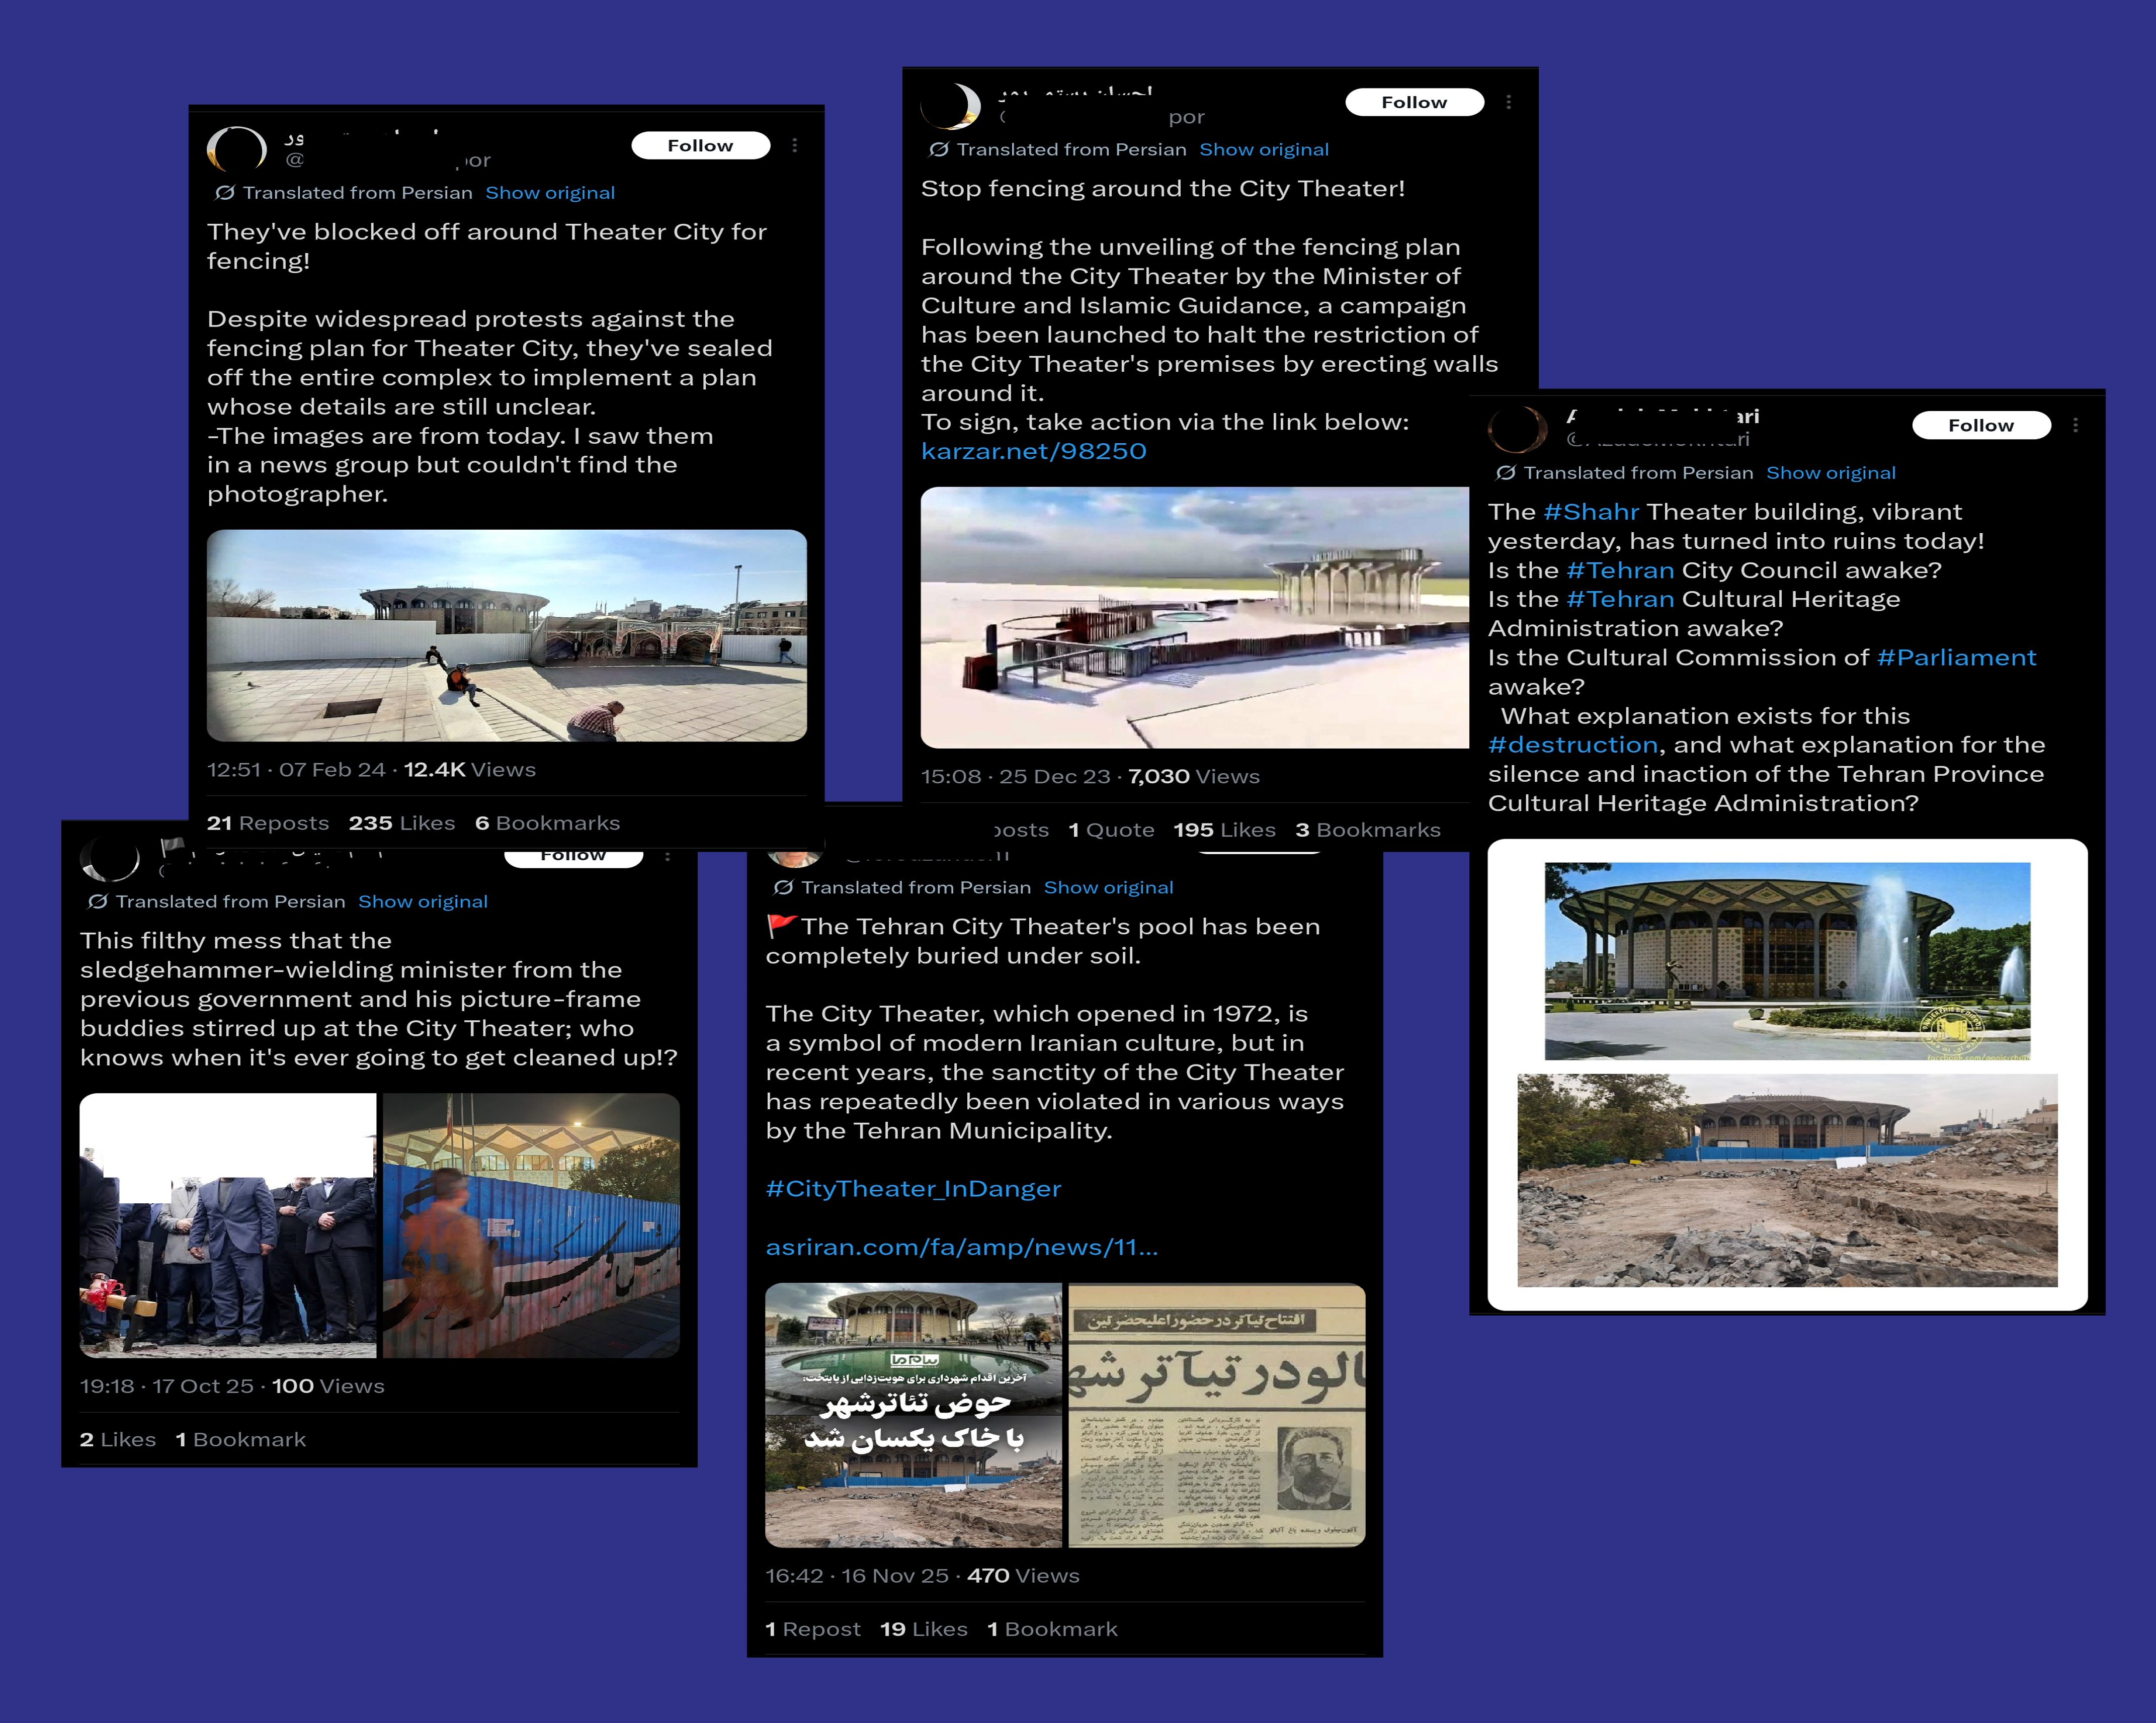
\includegraphics[keepaspectratio]{images/tweets.png}}

}

\caption{\emph{Figure 11. People sharing their opinions on X (Formerly
Twitter).\\
Sources: Forouzandeh1, 2025; Ehsanrostamipour, 2023 \& 2024;
Danielalefsefr, 2025; AzadehMokhtari, 2025.}}

\end{figure}%

The citizens expressed their concerns to the officials and the
municipality regarding the fence placement and the City Theater's
renovations on social media. However, the reconstruction project is
ongoing, and its end date remains unknown to the public. The users
shared some images of redesign proposals for the plaza and directly
addressed the matter of fence placement around the City Theater.

Even some users brought up the artistic and cultural legacy that the
City Theater has brought up since its foundation, with images of old
newspapers in the 1970s announcing the famous plays being performed at
the City Theater of Tehran (Fig. 11). This can reflect how prestigious
the City Theater space is to the public, how its preservation is
critical as a cultural and social heritage.

These are some examples of how the public encounters spatial
interventions through digital spaces to archive, review, evaluate, or
express, keeping themselves engaged with their city and urban life when
their voices are not actively heard.

\paragraph{Problem in a sentence}\label{problem-in-a-sentence}

Spatial memories are valuable insights into a space that are taken for
granted by designers/decision-makers in their interventions, leading to
the erasure of public space.

\newpage{}

\section{Research Objectives}\label{research-objectives}

In the era in which digital media has a vast impact on urban lives, it
even becomes an autonomous memorial archive (Haskins 2007). Having such
a large-scale, individual lived experience from citizens would help gain
a better understanding of citizens' reviews of urban environments. Also,
it's not only about opinions but about how they experienced the space
individually or collectively. This is a helpful step towards planning
and designing projects.

Also, within the right to the city notions (Harvey 2003; Lefebvre 1968),
it was discussed that memories of a space that holds dozens of lived
experiences from various individuals or groups turn the space into a
valuable environment, a place (Martin 2025). Having a place is not
limited to its physical existence, but also to how it's cloned in the
memories of those who interacted with it. This would be the link between
having the right to the city and having the right to the memory.

Having already expressed opinions or archived memories on open,
accessible platforms would aid designers and planners in studying a
citizen perspective and eventually find more efficient strategies for
public engagement (Williamson and Ruming 2020). The digital memory may
not be the final solution, but it will be a key starting point for many
urban transformations aiming to be more inclusive and plural.

The objectives can be defined as follows:

\begin{enumerate}
\def\labelenumi{\arabic{enumi}.}
\tightlist
\item
  Public engagement increases via virtual spaces (online digital
  platforms)
\item
  Inclusive design and planning
\item
  Digitally shared lived-experience validation as digital memories
  (right to the memory)
\item
  Design / Planning through urban data
\end{enumerate}

\section{Research Questions}\label{research-questions}

\subsection{Main Question}\label{main-question}

\textbf{How can digital memories shared by citizens help identify
spatial values as potential conditions for interventions in Teatré Shahr
Square?}

\subsubsection{Sub-questions}\label{sub-questions}

\begin{enumerate}
\def\labelenumi{\arabic{enumi}.}
\item
  How do digital memories narrate the lived experiences of citizens in
  the City Theater square on X (former Twitter) and Instagram?
\item
  What emotions can be traced from digital memories of City Theater
  Square?
\item
  What spatial qualities could be referred to from the shared emotions
  of City Theater Square?
\item
  What spatial values do citizens share about the City Theater square
  space transformation throughout time (before and after the latest
  intervention) as reflected on social media?
\item
  How can shared memories on social media inform design guidelines for
  the City Theater Square?
\end{enumerate}

To clarify how each sub-question will be addressed, the corresponding
methodology is briefly described in the following table.

\begin{longtable}[]{@{}
  >{\centering\arraybackslash}p{(\linewidth - 4\tabcolsep) * \real{0.5627}}
  >{\centering\arraybackslash}p{(\linewidth - 4\tabcolsep) * \real{0.0826}}
  >{\centering\arraybackslash}p{(\linewidth - 4\tabcolsep) * \real{0.3517}}@{}}
\caption{\emph{Table 2. Sub-questions classification and
methodology}}\tabularnewline
\toprule\noalign{}
\begin{minipage}[b]{\linewidth}\centering
Question
\end{minipage} & \begin{minipage}[b]{\linewidth}\centering
Type of analysis
\end{minipage} & \begin{minipage}[b]{\linewidth}\centering
Methodology
\end{minipage} \\
\midrule\noalign{}
\endfirsthead
\toprule\noalign{}
\begin{minipage}[b]{\linewidth}\centering
Question
\end{minipage} & \begin{minipage}[b]{\linewidth}\centering
Type of analysis
\end{minipage} & \begin{minipage}[b]{\linewidth}\centering
Methodology
\end{minipage} \\
\midrule\noalign{}
\endhead
\bottomrule\noalign{}
\endlastfoot
\begin{minipage}[t]{\linewidth}\centering
\begin{enumerate}
\def\labelenumi{\arabic{enumi}.}
\tightlist
\item
  How do digital memories narrate the lived experiences of citizens in
  the City Theater square on X (former Twitter) and Instagram?
\end{enumerate}
\end{minipage} & Descriptive / Analytical &
\begin{minipage}[t]{\linewidth}\centering
Literature review,\\
Data collection using scraping apps as strings of text, Topic
modelling\strut
\end{minipage} \\
\begin{minipage}[t]{\linewidth}\centering
\begin{enumerate}
\def\labelenumi{\arabic{enumi}.}
\setcounter{enumi}{1}
\tightlist
\item
  What emotions can be traced from digital memories of City Theater
  Square?
\end{enumerate}
\end{minipage} & Descriptive / Analytical & Sentiment analysis to
recognize and classify emotions from texts extracted from Tweets and
Instagram posts \\
\begin{minipage}[t]{\linewidth}\centering
\begin{enumerate}
\def\labelenumi{\arabic{enumi}.}
\setcounter{enumi}{2}
\tightlist
\item
  What spatial qualities could be referred to from the shared emotions?
\end{enumerate}
\end{minipage} & Descriptive / Analytical & Locating the spatial
features referred to by emotions through cognitive indicators \\
\begin{minipage}[t]{\linewidth}\centering
\begin{enumerate}
\def\labelenumi{\arabic{enumi}.}
\setcounter{enumi}{3}
\tightlist
\item
  What spatial values do citizens share about the City Theater square
  space transformation throughout time (before and after the latest
  intervention) as reflected on social media?
\end{enumerate}
\end{minipage} & Normative & Classifying the values of spatial features
referred to by emotions into positive and negative \\
\begin{minipage}[t]{\linewidth}\centering
\begin{enumerate}
\def\labelenumi{\arabic{enumi}.}
\setcounter{enumi}{4}
\tightlist
\item
  How can shared memories on social media inform design guidelines for
  the City Theater Square?
\end{enumerate}
\end{minipage} & Normative & Creating design guidelines based on spatial
qualities and interventions corresponding to negative spatial values \\
\end{longtable}

\newpage{}

\section{Scope (Case Study)}\label{scope-case-study}

\subsection{City Theater Plaza}\label{teatruxe9-shahr-city-theater}

The reason for choosing this specific public space is not only its
architectural quality, but also its historical legacy, which holds many
urban events, activities, and daily-life patterns. A public space at the
heart of the Iranian capital, Tehran, has always been a focal point for
its dwellers.

\begin{figure}[H]

{\centering \pandocbounded{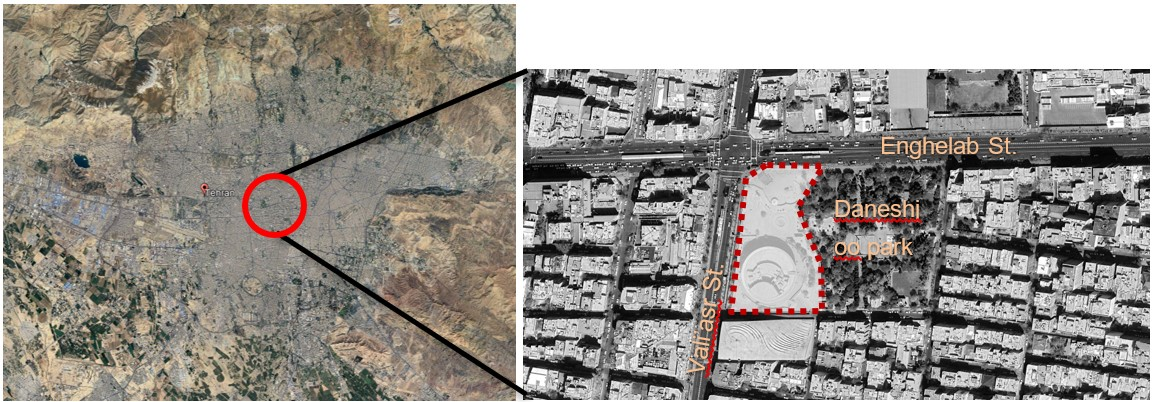
\includegraphics[keepaspectratio]{images/teatre shahr.jpg}}

}

\caption{\emph{Figure 12. Tehran's overview and City Theater's location
within it.\\
Source: Google Earth, 2024.}}

\end{figure}%

Thus, it holds a large scale of digital memories within itself, which it
collects and studies. Also, because there is no explicit online platform
for citizens to share their digital memories of a specific urban space,
the current study focuses on the most popular and recognized public
space. This will increase the likelihood of related data being available
and collected.

\subsection[X and Instagram]{\texorpdfstring{X and
Instagram\footnote{Since the mentioned social media platforms are
  officially banned in Iran, there aren't precise data or information
  regarding the user accounts in Iran. The current descriptions are
  based on the author's experiences who was born and raised in Iran
  using the mentioned social media platforms that are popular among the
  existing internet users who access them via VPNs that change their IP
  addresses in Iran.}}{X and Instagram}}\label{x-and-instagram4}

Multiple social media platforms hold vast amounts of data about digital
memories. In the Iranian case, users are mostly active on the two
platforms, X (formerly Twitter) and Meta's Instagram. The X has always
been one of the most dynamic platforms for Iranians to share their
opinions on the state of the country and their daily lives. Instagram is
the most popular social media platform among Iranians, with a 28.33\%
share, and X holds 5.4\% over the last decade (Dec 2015 - Dec 2025)
(statcounter, n.d.). X may not be the most popular platform, but it's
where many users share their opinions on critical or general topics more
straightforwardly and transparently. While other platforms like
Instagram, Facebook, or Pinterest focus on sharing media and general
descriptions, X would offer more textual content that conveys a stronger
sense of individual or professional positionality regarding a topic.

Based on these reasons, X and Instagram are chosen as the targeted
social media platforms to collect their digital memories of City Theater
Square and to analyze the textsin tweets and Instagram posts.

\newpage{}

\section{Literature Review
(Relevance)}\label{literature-review-relevance}

\subsubsection{Right to the memory as a right to the
city}\label{right-to-the-memory-as-a-right-to-the-city}

The Right to the City was coined by the French philosopherHenri Lefebvre
in the era when social movements became viral among young intellectuals
and labor activists seeking social justice in urban areas (Mitchell
2003). After Modernism, the ownership of land in urban areas through
capitalist monopoly expanded dramatically. At that time, politicians,
social activists, urbanists, and philosophers realized the need for a
just city and a~healthy environment between the city blocks is something
crucial and, in other words, could be considered a right for the
citizens who live in there and use its space (Habibi and Amiri 2016;
Harvey 2015; Lefebvre 1968).

Furthermore, the notion was developed by Harvey (2015), who argued that
city dwellers can fight for their rights over space and, more generally,
over the city. This act works against the manipulation and trespassing
in the public domain by private developers and governments who attempt
to impose capitalism across vacant spaces for profit. Harvey (2015)
suggested that the public could prevent this through social activities
and demonstrations by recognizing the Right to the City as their
individual will to change their living space and ultimatelythemselves.
Thus, the Right to the City is mostly interpreted as the right to public
space. Who has access to it and who doesn't defines this right (Harvey
2015; Habibi and Amiri 2016; Moroni and Chiodelli 2014).

Suppose we consider the right over public space derived from the concept
of the right to the city. Once people have lived experiences in a space,
it forms their memories of that space. Since memory and physical space
can be imagined as intertwined, memories are attached to physical space.
In contrast, the space holds the memories within its boundaries(notions
of sense of place, etc.). Thus, having the right to a public space
automatically grants the right to its memories at the same time. In
other words, policy makers, designers, or any other entity that holds
the authority or power to change the space must take into account the
sensitivity of a public space, not only based on general spatial values
and qualities, but also on memories embedded in that space. It should be
acknowledged that citizens have a right to the space and to their
memories of it as common goods, too.

Based on the same theoretical principles, Harvey (1993) has always
discussed the right to the city as extending beyond mere access
toresources (Harvey (1993) as cited in Tedeschi 2024).

The abstract space described by Lefebvre (1991), limited to planning and
design perspectives, has changed into a rapid representation in various
forms through digital information. The space is no longer an abstraction
of a physical entity; it is regenerated and transformed in a digital
domain based onrapidly changing information (Lefebvre (1991) as cited in
Shaw and Graham 2017).

The technological development has brought new definitions of the right
to the city concept. Tedeschi (2024) argues that algorithms have a right
to space, as they rapidly produce and update information about physical
space. This makes the accessibility and experience for its dwellers
either disruptive or reinforcing, leading them to negotiate their social
interactions and power over space with this non-human entity. This
creates a different level of inequality in a digital dimension.

\subsubsection{Digital era (archival
memories)}\label{digital-era-archival-memories}

In the digital age, the media has become a tool for any individual to
express their thoughts, share their feelings, raise ideas, share
experiences and memories, or cry out for their rights as critical
matters. One major feature of digital media is their archival potential.
They are the database of memories of many individual and collective
activities or events in a variety of contexts.

What archival memories can bring is not comparable to a curated,
centrally organised museum set up exclusively for visitors, but to an
independent, multi-voice platform that anyone with a digital device can
share and publish to other users throughout the internet (Haskins 2007).
Even such an idea was suggested by Lefebvre (2003, as cited in Tedeschi
(2024)): having a self-management feature on a digital platform should
be a right, even though it was considered a right to urban resources
rather than something higher.

The importance of the digital domain is not just about having horizontal
archival memories created by numerous individuals, but about the digital
space itself as a phenomenon that can trace the contents of a society in
a physical space. Shaw and Graham (2017, 909) brings up the importance
of data flows in urban studies:

\begin{quote}
``\emph{Just as the urbanization of water is a processional notion which
can uncover `stories about the city's structure and development', so can
a reading of the city's `political, social, and economic conduits'
through which information flows also ``carry the potential for an
improved, more just, and more equitable right to the city''}''
\end{quote}

The data flows of urban life have the potential to reflect many aspects
of the city's dynamics, struggles, and synergies throughout its history.
Not only the past, but also, thanks to real-time communications, the
present state of the city. Solnit (2001, 91) also points out the
historical importance of urban space, or more precisely, the streets, as
\emph{``repositories of history''} that are lived in. The lived
experiences within these repositories can be shared and recorded on
social networks as valued, recognized spaces that hold history.

\subsubsection{Public Engagement (digital
participation)}\label{public-engagement-digital-participation}

Again, from the right to the city, Mitchell (2003) highlights the right
to the city, which is \emph{oeuvre}\footnote{A piece of art {[}in
  French{]}}, a piece of art, that each citizen contributes to (Tedeschi
2024, 3). It is a piece of art, like a tapestry, with which city
dwellers can create by sharing their lived experiences and turn those
experiences into action (Tedeschi 2024, 6; Currie, Knox, and Mcgregor
2022; Martin 2025). Taking citizens' lived experiences and emotions into
account in the planning and design process would lead to a valued space,
or the so-called place (Martin 2025). Moreover, public participation has
always been better received in urban projects, regardless of their
effectiveness (Martin 2025).

Even reframing the Right to the City leads to co-design from a
governmental perspective to shape public space rather than just having
citizens gain more power and rights over their space (Tedeschi 2024).

Based on the notions explained about archival media, autonomous
authorship would lead todemocratized media (Haskins 2007; Martin 2025).
This can be recognized as the first steps towards public participation
before engaging the stakeholders, mostly citizens or vulnerable groups.
To understand the extent of participation, Arnstein (2019) proposed the
concept of ``The Ladder of Participation,'' which describes the levels
of public engagement and participation as a ladder with progressively
higher levels. The ladder starts with the least level of participation,
known as Therapy, and culminates in the ultimate form of active citizen
engagement in the design process.

Based on Arnstein (2019)`s ladder of participation, having citizens'
shared lived experiences on digital platforms may be a lower step, yet a
passively engaging position that needs updating. Because this is not
about the planner/designer's active interaction with citizens, but about
reading or tracing citizens' emotions from an autonomous, semi-survey
publicly available (Martin 2025).

One positive aspect of having the digital inputs is the large scale of
data. Despite usually having a limited number of active participants in
urban projects, digital platforms offer the opportunity to gather
qualitative insights from a broader range of citizens(Martin 2025;
Fathullah and Willis 2018).

Digital participation is also supported by various studies (Martin 2025;
Haskins 2007). Also, Williamson and Ruming (2020) points out a further
step: using social media data on a participatory scale. They suggested
the term `Frontloading', which refers to engaging stakeholders in the
early stages of planning by accessingshared emotions and experiences on
social media. (Read through \#MySydney case)

\newpage{}

\section{Conceptual Framework}\label{conceptual-framework}

The conceptual framework will help identify the necessary criteria for
running sentiment analysis on the collectedtext strings from the
targeted platforms. The conceptual framework is based on the principles
derived from the literature review, considering the spatial qualities
that shape how a space evokes memories and lived experiences for
citizens when they interact with it. And, how this can be identified and
classified through semantic analysis of string data on online platforms.

The initial concept would be the transformation of space into place
through people's interactions, which shape their sense of belonging to
their environment based on several spatial and contextual factors
(Martin 2025).

\begin{figure}[H]

{\centering \pandocbounded{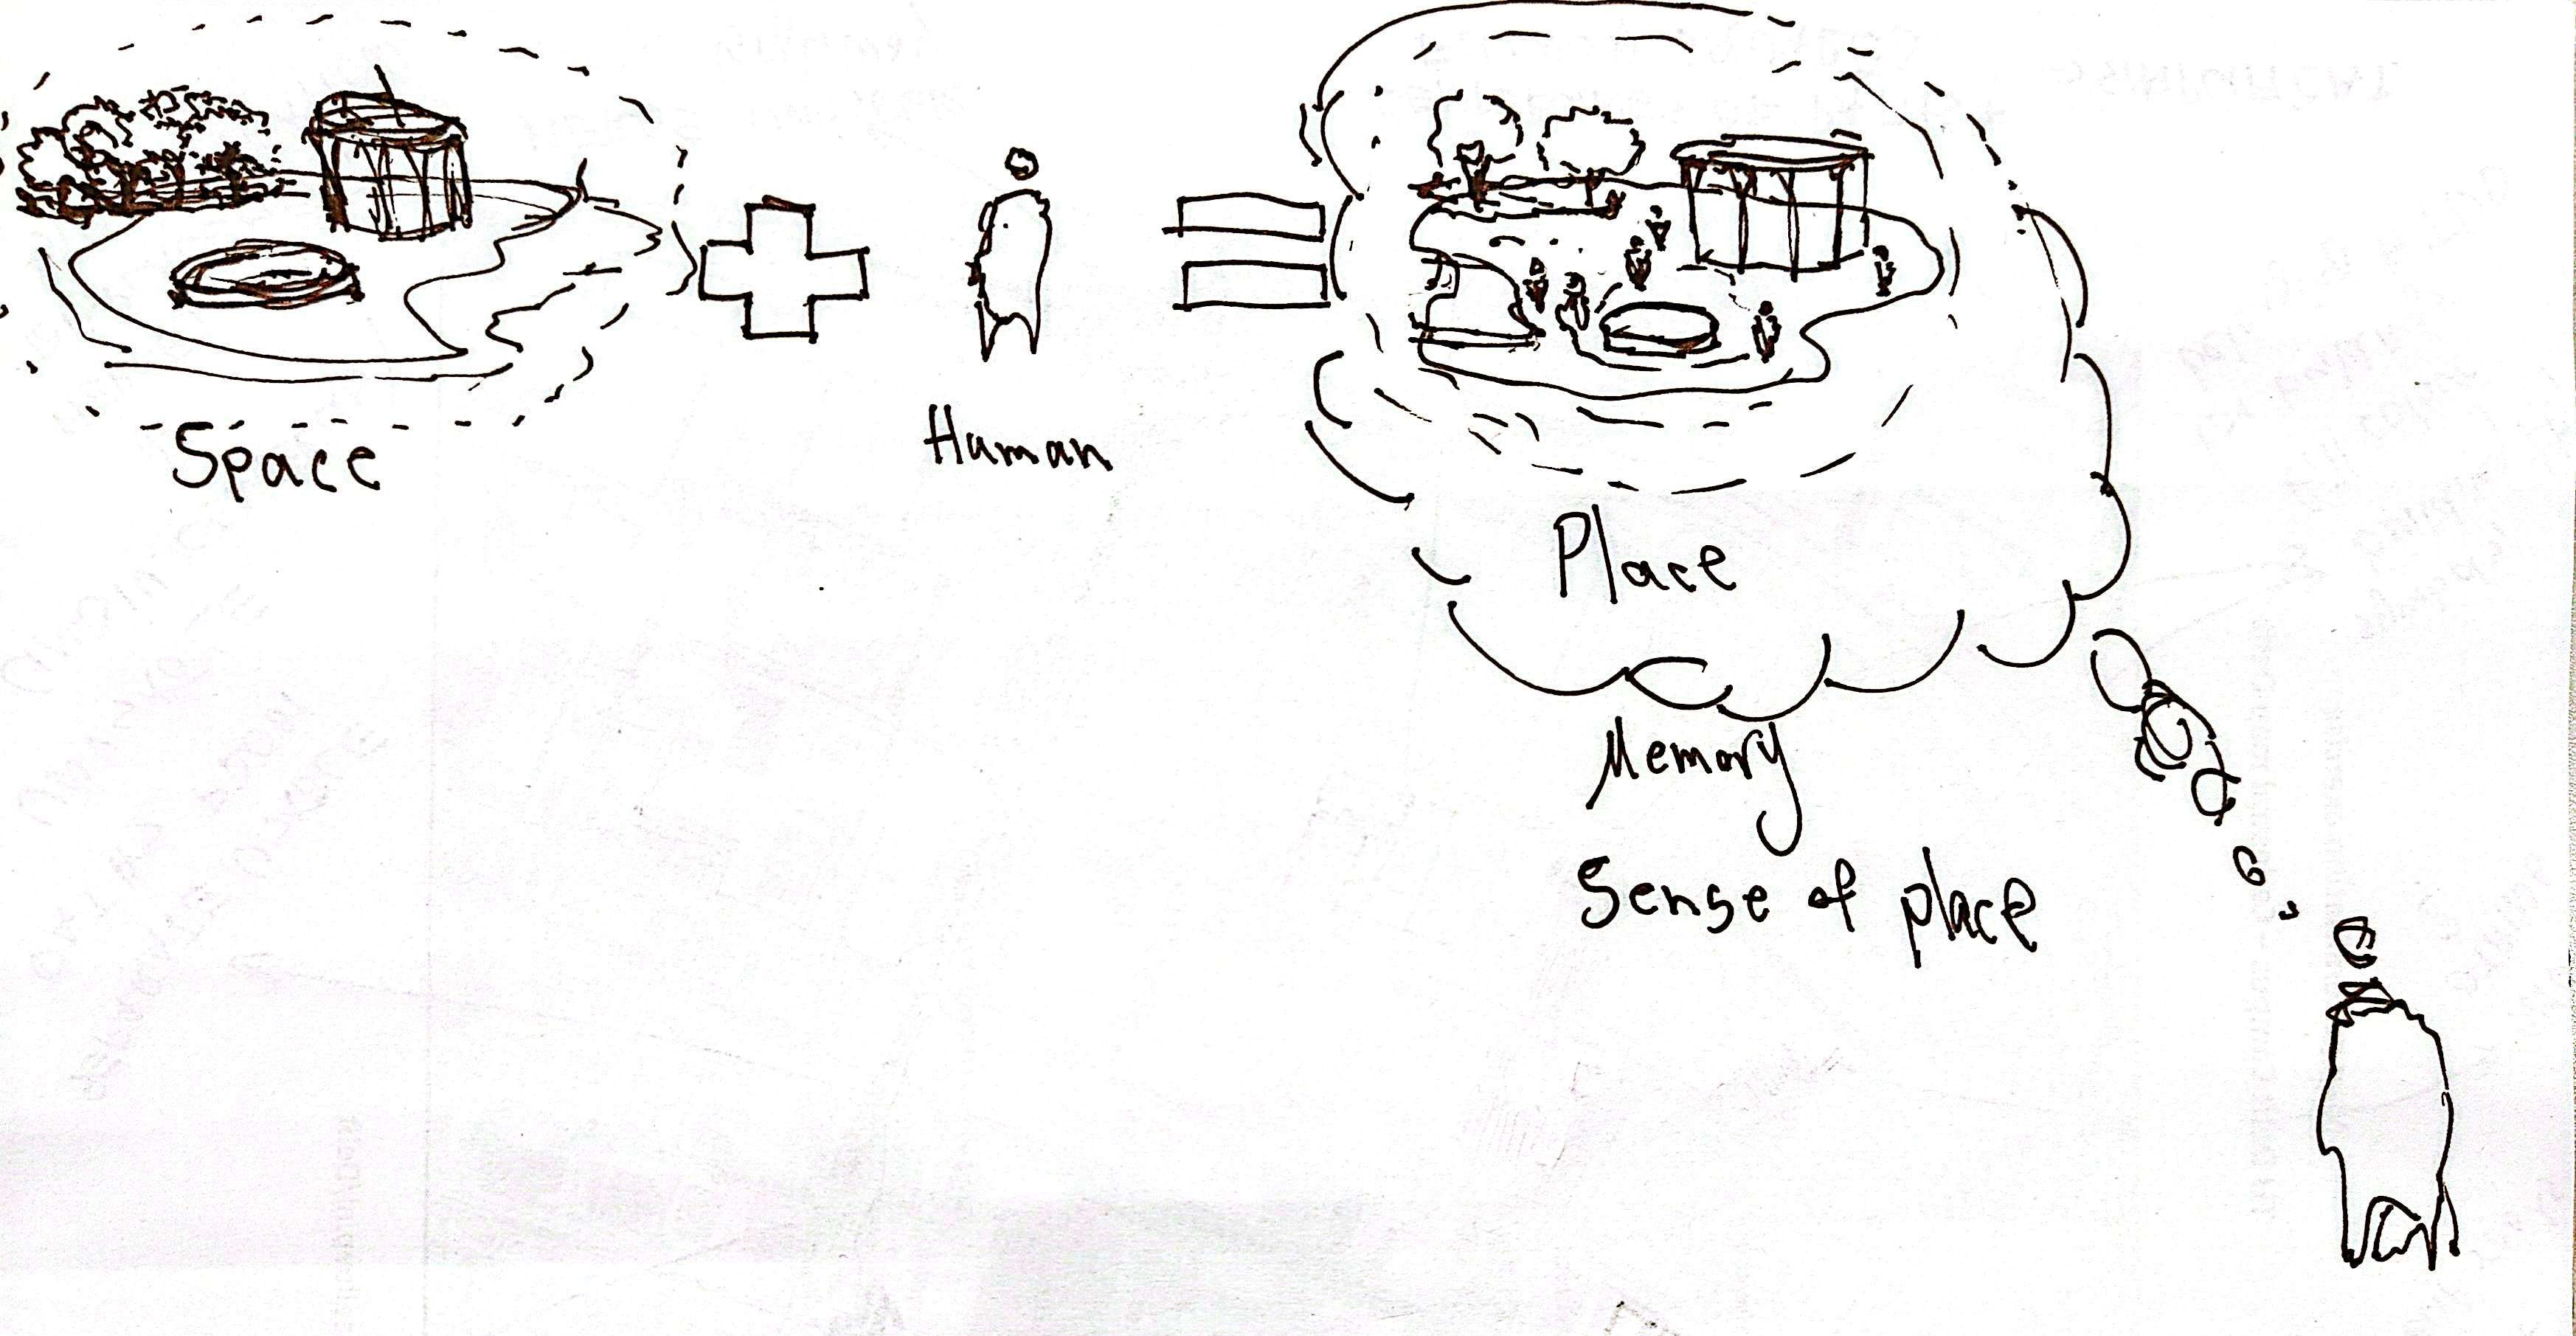
\includegraphics[keepaspectratio]{images/CamScanner 12-19-2024 19.48_10-01.jpg}}

}

\caption{\emph{Figure 13. Space to place the transformation Diagram}}

\end{figure}%

The belonging factors can be identified in Fig. 4 below, which
represents a very initial draft of the spatial and contextual aspects
that would have a direct and indirect impact on one's sense of belonging
to the environment in which they have been and interacted.

\begin{figure}[H]

{\centering \pandocbounded{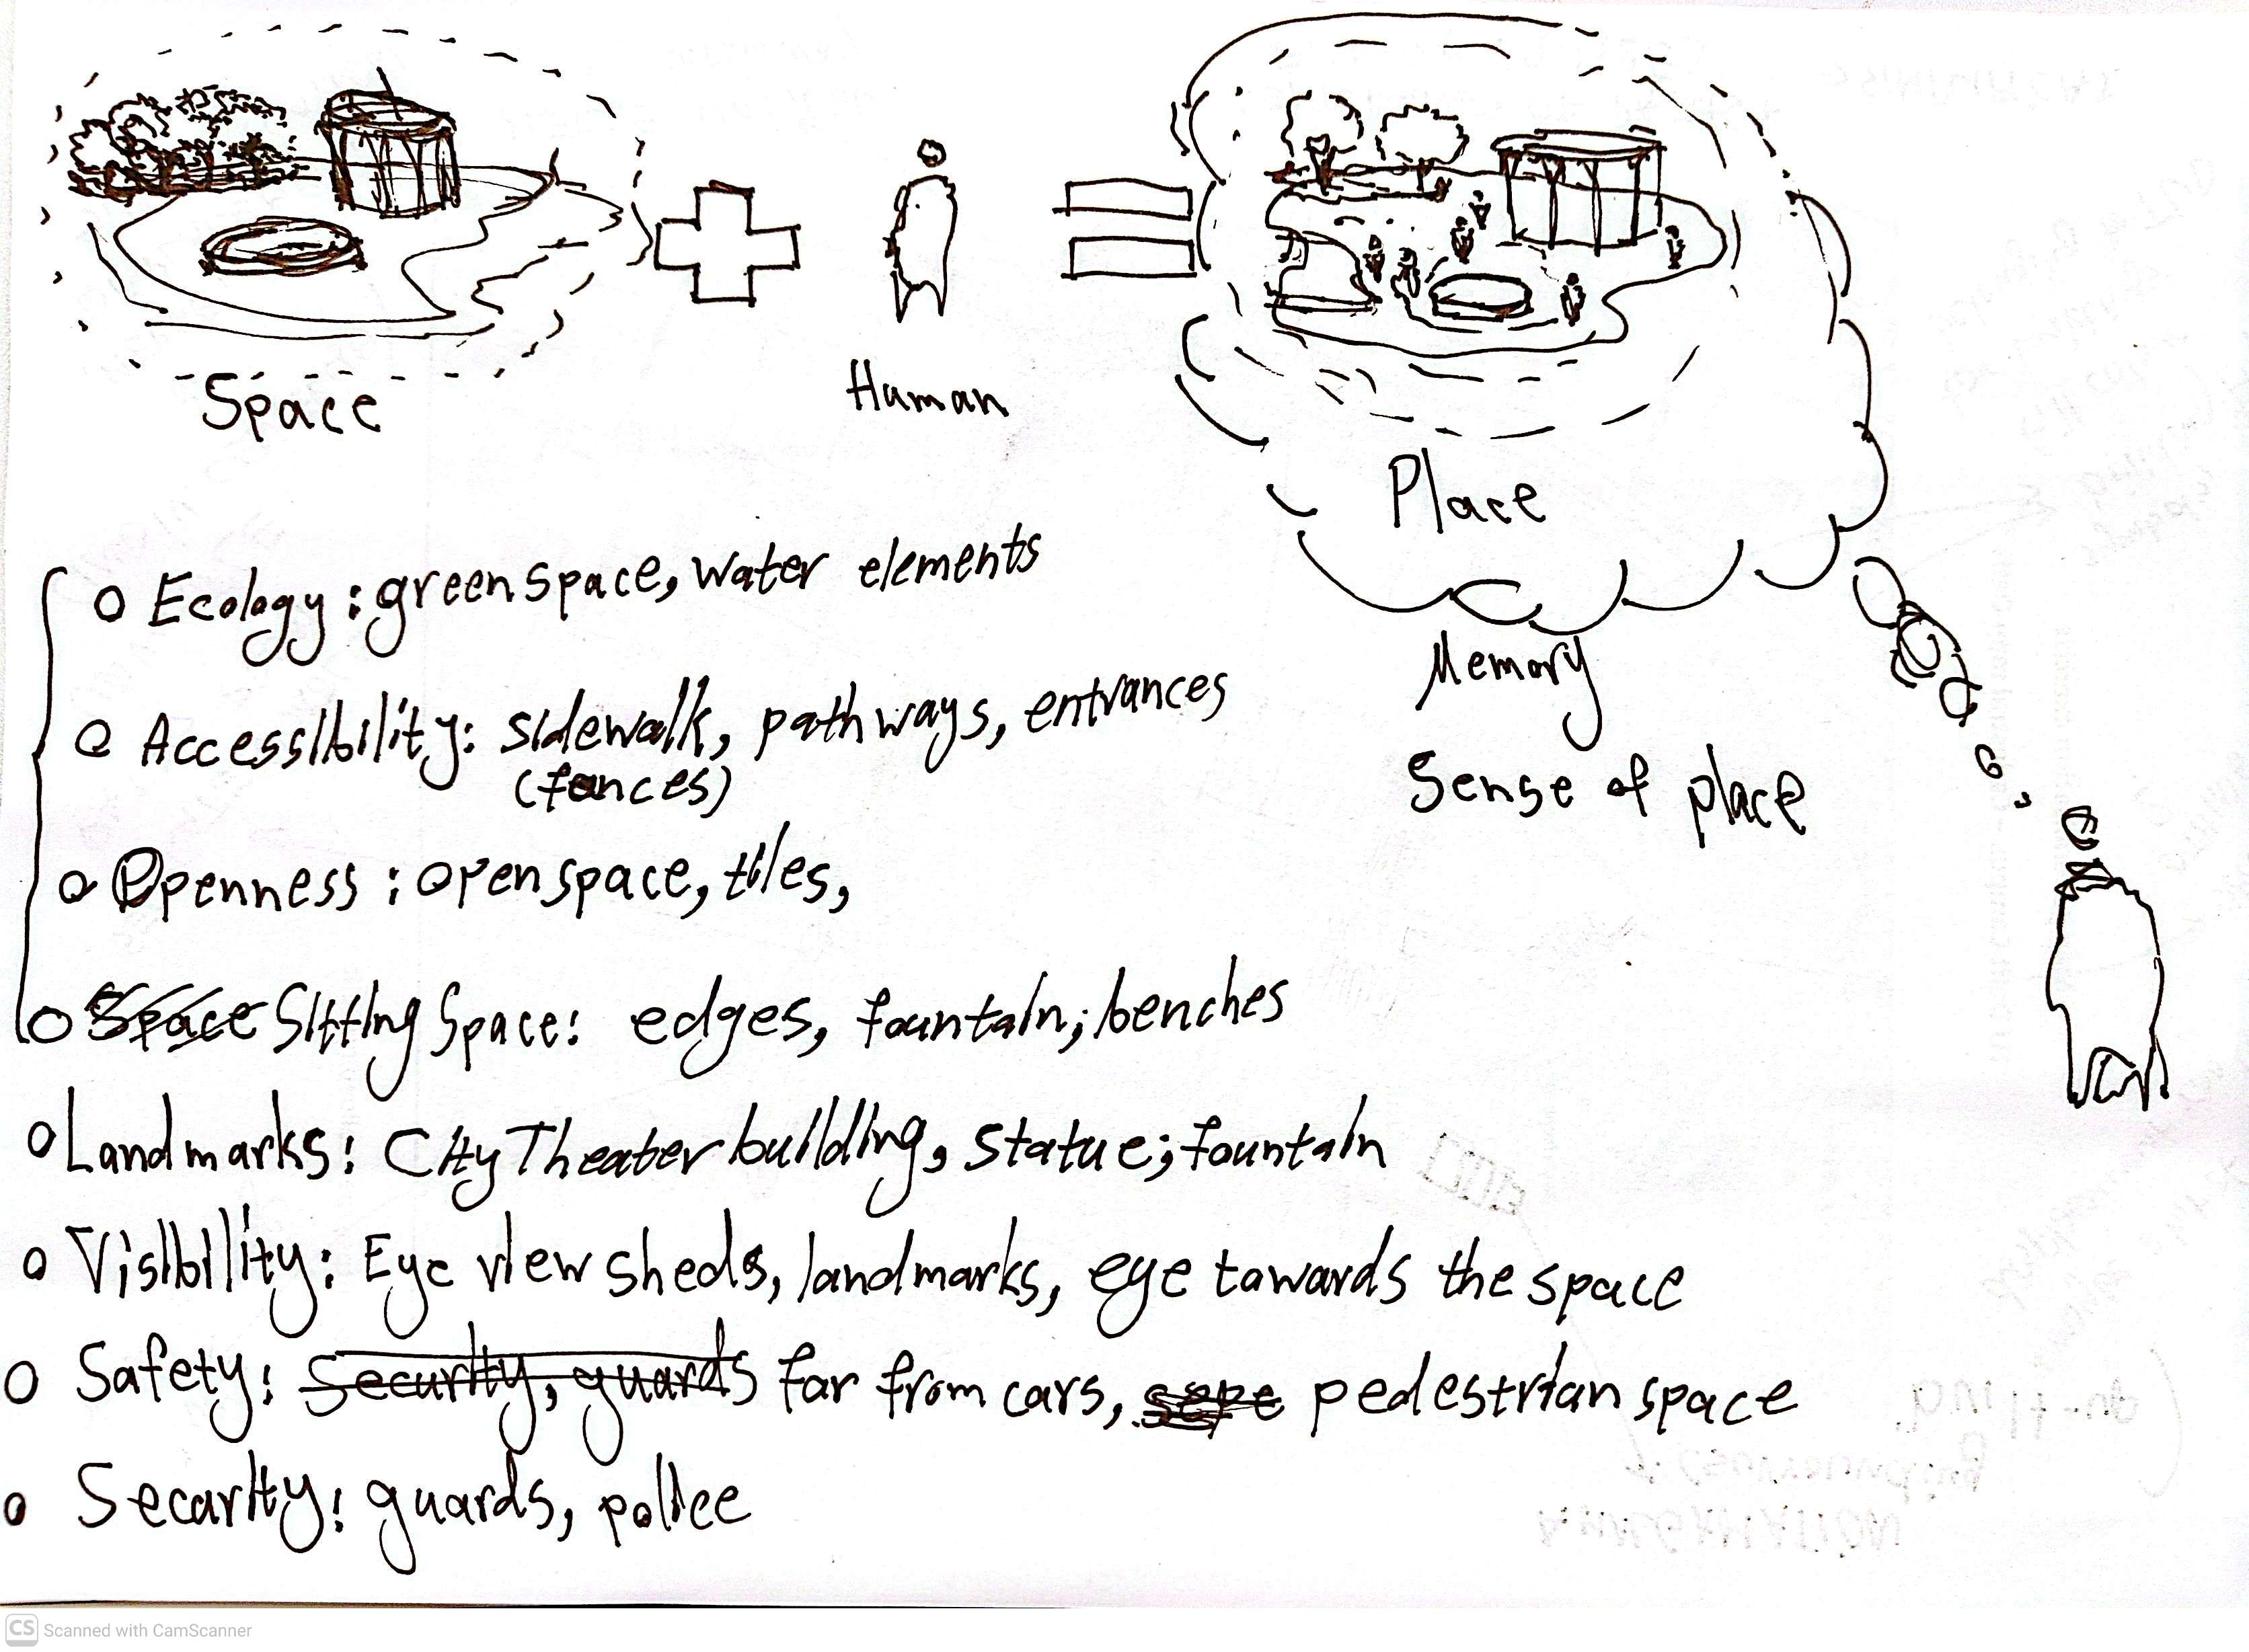
\includegraphics[keepaspectratio]{images/CamScanner 12-19-2024 19.48_9.jpg}}

}

\caption{\emph{Figure 14. Sense of belonging, spatial and contextual
affecting factors}}

\end{figure}%

\begin{itemize}
\item
  Ecology: green \& blue elements, living species
\item
  Accessibility: sidewalk, pathways, entrances, gateways
\item
  Openness: open space, tiling, profile details
\item
  Sitting space: edges, fountain, benches
\item
  Landmarks: City Theater building, statues, and a fountain
\item
  Visibility: Eye view sheds, landmarks, corridors,
\item
  Safety: pedestrian priority, traffic control
\item
  Security: active presence, observer eye (eyes on the street)
\item
  Geography: topography, location
\item
  Climate: temperature, humidity, sun angle
\item
  Identity: symbols, culture, language, lifestyle
\end{itemize}

The memories of space or place that are turned into lived experience and
expressed through emotions in digital space are useful for analyzing a
space from a cognitive perspective.

Users share different experiences of their presence and interactions
within the lived space on social media. As mentioned before, their posts
and tweets would hold various emotions. The main gap is how to trace the
spatial feature from these shared emotions.

Thanks to Lynch (1964)'s cognitive analysis concepts and methods of the
perceived space or city, the spatial features could be tracked and
recognized by how the individuals described their situation or position
of the space, and their mentions could be classified into Lynch's
cognitive features of nodes, lines, areas, edges, and landmarks. The
subsequent workflow would focus on relating different sentiments to
their corresponding spatial features in the context. For example,
someone could have gotten angry due to the presence of edges in a
specific area.

The sentiment classification of each feature would help identify
valuable places and how they were designed, with a corresponding design
for the public that results in livability and placemaking. Also, spaces
that need improvement will be identified. Based on the feelings that
address the specific feature, the association between physical space and
emotions in memory will result in positive or negative values. This
would help with the further steps of the design process and with
producing spatial conditions in spaces that hold memories that can be
recalled as a public good.

\newpage{}

\subsection{Framework}\label{framework}

Furthermore, to integrate the adapted concepts from the literature
review, as a guiding theme for the research and design process, a
conceptual framework was illustrated in the following diagram.

\begin{figure}

{\centering \pandocbounded{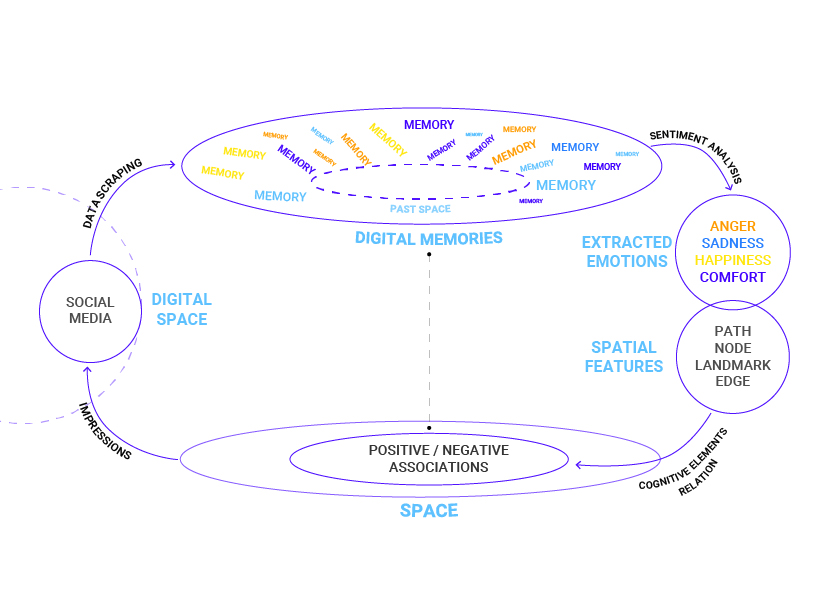
\includegraphics[keepaspectratio]{images/Artboard 3-100.jpg}}

}

\caption{\emph{Figure 15. Conceptual Framework}}

\end{figure}%

The diagram depicts the three main concepts of the study, social media,
digital memory, and space, and how they are related to each other based
on the defined methods and processes.

\subsubsection{Definitions and
processes}\label{definitions-and-processes}

\textbf{Space:} The existing physical space that, in this case, can be
considered as the public space, or to be precise, City Theater's plaza
in Tehran, which holds various activities, spatial elements, and
mobility within. Users of social media interact with the space. The
result of this interaction is expressed in another sphere by them.

\textbf{Social Media:} Social media is a fragment of a larger sphere,
the digital space, that includes many other domains with various
activities, characteristics, and users. The study's focus is on social
media platforms (i.e., X \& Instagram) where users share their
expressions, opinions, attachments, and, in general, their lived
experience of the space as a memory. These memories are shared as Tweets
and Instagram posts with footage, images, or plain descriptions. These
data will be scraped from their platforms as text strings (only the
textual contents) that address the space with the keywords City Theater
or City Theater's intersection to be collected.

\textbf{Digital Memories:} The scraped and collected data are literally
the memories of the space in the past (or, as it is called, the past
space). Any of the memories refers to the space. But that's not all of
the input. Each of them holds a specific expression, for it is a
personal experience. The various memories can be classified by how they
were expressed, along with one or more emotions.

\textbf{Extracted Emotions:} The emotions within digital memories can be
extracted and classified using sentiment analysis. The emotions in
digital memories will be identified from textual expressions. Each word
or phrase addresses a feeling or experience that can be classified into
the following items:

\begin{enumerate}
\def\labelenumi{\arabic{enumi}.}
\item
  Anger
\item
  Sadness
\item
  Comfort
\item
  Happiness
\end{enumerate}

Having these classes, the emotions can be categorized as negative or
positive feelings.

\begin{longtable}[]{@{}cc@{}}
\caption{\emph{Table 3. Categories and Classifications of
Emotions}}\tabularnewline
\toprule\noalign{}
Emotion Categories & Value Classification \\
\midrule\noalign{}
\endfirsthead
\toprule\noalign{}
Emotion Categories & Value Classification \\
\midrule\noalign{}
\endhead
\bottomrule\noalign{}
\endlastfoot
Anger & Negative \\
Sadness & Negative \\
Comfort & Positive \\
Happiness & Positive \\
\end{longtable}

\textbf{Spatial Features:} Based on Lynch (1964) 's perceptual urban
elements, each shared emotion would have one or more corresponding
spatial features that affected the person's cognition and co-created
their lived experience. The features are as follows:

\begin{enumerate}
\def\labelenumi{\arabic{enumi}.}
\tightlist
\item
  Path
\item
  Node
\item
  Edge
\item
  District (areas with common character)
\item
  Landmark
\end{enumerate}

\begin{figure}

{\centering 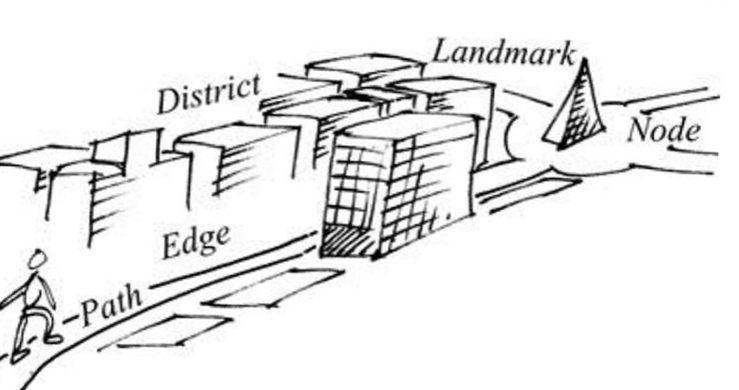
\includegraphics[width=4.16667in,height=\textheight,keepaspectratio]{images/interactionofelement-2-e1569672351975.jpg}

}

\caption{\emph{Figure 15. Lynch's cognitive urban elements from `The
Image of the City'.\\
Source: Semanur Can, 2026.}}

\end{figure}%

The urban elements are addressed, directly or indirectly, by users in
their digital memories. This addressing comes with an evaluation of
their emotions towards the spatial features. Based on this and the
extracted emotions, the negative and positive ratings can be linked to
the corresponding urban elementsrecognized mentally by the valuers. This
relational process helps create positive or negative associations within
the space.

\textbf{Positive/Negative Associations:} The associations made through
the relational process will reveal spatial features with negative or
positive values. Features with negative ratings require improvements and
interventions. While the ones with positive ratings might have design
qualities to be recognized, preserved, or reused through interventions
within the space, the original context of this study is.

Overall, as shown in \hyperref[conceptual_frame]{Fig. 15}, the cycle can
continue in the original space after the interventions based on
positive/negative associations are applied. The transformed spatial
features within the space can make an impression on their valuers,
shaping their lived experience of the space again. Therefore, as
impressions accumulate, a sense of place builds as it moves through the
space and its elements. The impressions emerge in different forms, such
as Tweets and Instagram posts, regarding the physical space sphere. In
that way, the impressions of the physical space are transferred to the
digital space (i.e., social media) and create a clone of the existing
space.

The past, the transforming, and the existing space are not shaped
onlymentally. But also, that mental recognition of space is represented
in social media, shared within the digital space.

\newpage{}

\section{Methodology (methods and
planning)}\label{methodology-methods-and-planning}

The main target is to collect data from posts and tweets shared by
public profiles on Instagram and X (formerly Twitter). The analysis will
focus on the latest interventions in City Theater Square. There are
pre-intervention and post-intervention phases in which the public shared
their opinions, expressions, and impressions as lived experiences, both
when the square was intact and when it was transformed through redesign
procedures over the past two years of a time-stretched project
(Aleksandar et al., n.d.).

The main variable that will be collected is the text strings within
tweets on X and post captions on Instagram, using a scraping application
specialized for these platforms \footnote{Tweet scraper V2-X for Twitter
  and Instagram scraper} considering the legal and regulatory procedures
of online scraping. The data collection will follow the specified time
frame mentioned previously and usedefined keywords to narrow the search
domain as specifically as possible. Names like ``Teatré Shahr'',
``Teatré Shahr square'', or ``Vali'asr intersection'' would be used as
keywords to identify and collect any related text data to the chosen
case study(Williamson and Ruming 2020).

After that, the data needed to be cleaned of unnecessary details and
irrelevant expressions so the analysis could be applied appropriately.
The unnecessary details include personal information and opinions on
highly sensitive topics that may cause risk to data subjects. The
necessary data would include sentiments, spatial features, and memorial
expressions related to the space (i.e., City Theater and its
surroundings), all in string format. After that, the cleaned data will
be classified based on sentiment values derived from the structured
conceptual framework, using qualitative content analysis(Williamson and
Ruming 2020). By overlapping the driven criteria with semantically
classified data, classified as various expressions of anger, sadness,
happiness, fear, etc., the spatial qualities and design guiding values
could be shaped or at least frame an overview of what is valuable and
should be preserved, and what might be the alternatives of design for
such public spaces.

\subsection{Methodological Framework}\label{methodological-framework}

Based on the above-mentioned notions and theoretical backgrounds, the
conceptual framework is structured, serving as a theoretical lens for
the methodology and subsequent steps of this study. The details and
connections of each notion are illustrated in the following figure.

\begin{figure}

{\centering \pandocbounded{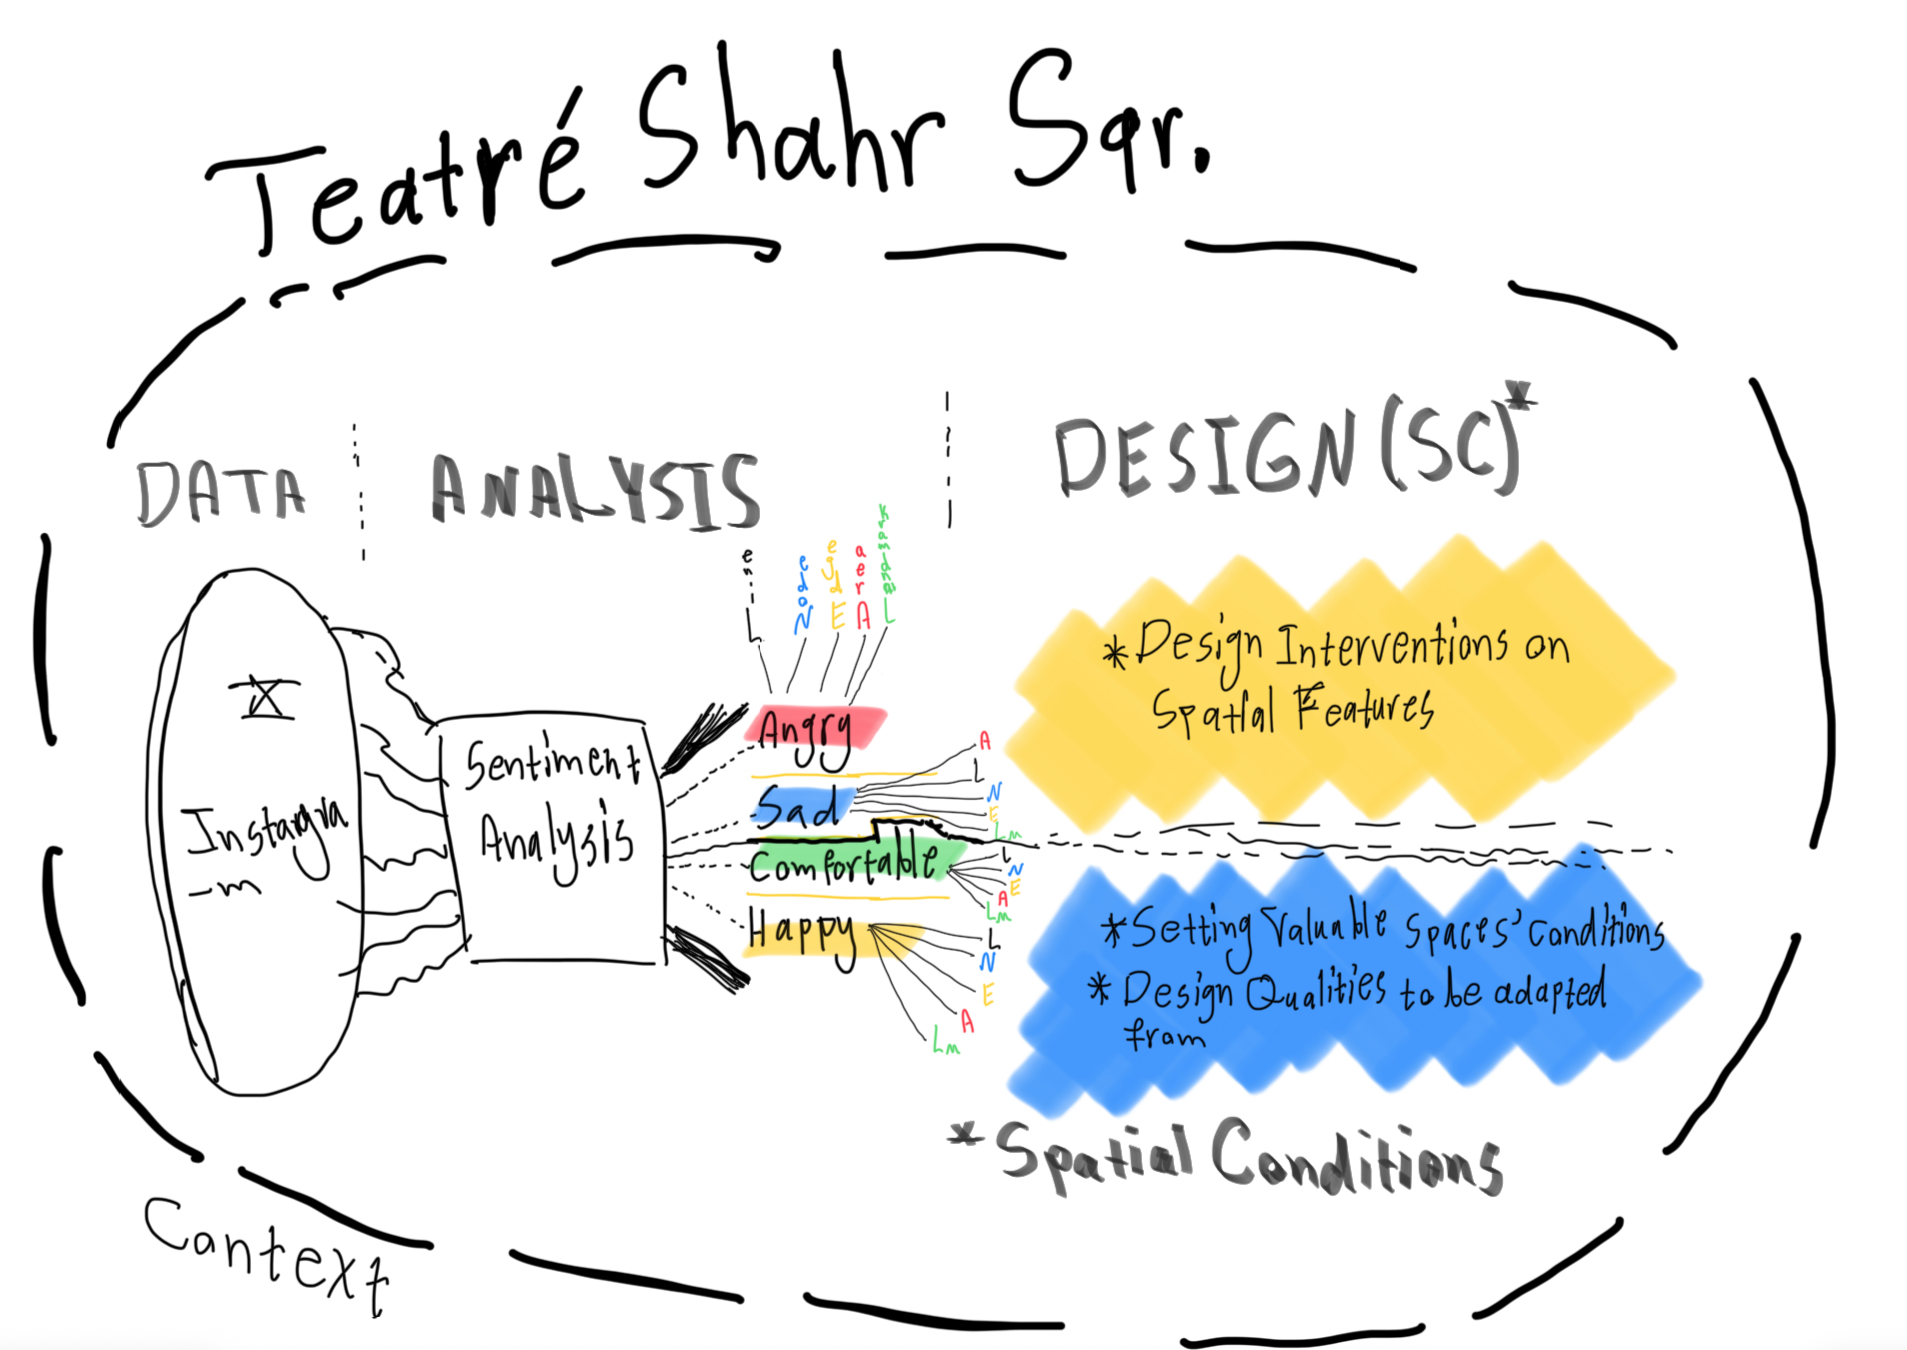
\includegraphics[keepaspectratio]{images/Screenshot 2026-01-11 at 19.05.48.png}}

}

\caption{\emph{Figure 16. Methodological Framework.}}

\end{figure}%

Starting with social media, the data in Tweets and Instagram posts is
rooted in the virtual digital space and can be traced back todigital
memories. That is the second sphere, which holds the lived experiences
within the texts, extracted as emotions using sentiment analysis. Four
main considered emotions also refer to spatial features that can be
identified using the cognitive approaches. The space is perceived as
simple objects such as lines, nodes, and landmarks. Not only do the
emotions address each spatial feature, but they also evaluate it. There
are physical elements that may have negative effects (Angry or Sad) or
positive effects (Happy or Comfortable) on people experiencing their
interaction with the space, and they rate them by expressing
emotionsstored as digital memories.

After relating each emotion to its addressed physical elements within
the space, emotions such as anger or sadness can be considered spaces
that do not properly correspond to the public. Thus, they may need
spatial improvements or interventions. The second approach would focus
on spaces that evoke happiness or comfort among users on social media.
Those spaces are already public spaces and contribute to the space's
livability. They can be considered valuable spaces, while their spatial
characteristics should be processed and applied as design qualities in
spaces that do not possess the same qualities within Teatré Shahr
square. All of this process happens within its context, which is Teatré
Shahr in this case, and each step has interrelations with the
environment chosen as the study area. Hopefully, in the design steps,
the relationship would be circular rather than one-way and more
interactive.

\newpage{}

\subsection{Expected Outcomes}\label{expected-outcomes}

The expected outcomes are considered to be either the results of data
analysis, spatial design guidelines, or interventions on the case study,
aka Teatré Shahr square.

\begin{figure}

{\centering 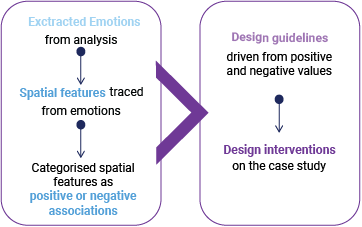
\includegraphics[width=5.20833in,height=\textheight,keepaspectratio]{images/Expected Outcomes.png}

}

\caption{\emph{Figure 17. Expected Outcomes.}}

\end{figure}%

The outcomes would be categorized into results of sentiment analysis of
text strings collected from tweets, serving as an archive of emotions,
along with their linked spatial features, matchedbased on cognitive
indicators of urban space perception. This leads to valuing spatial
features based on emotions as eithernegative or positive elements within
the space. These values will be localized based on their in-text
descriptions of the space in the form of hand drawings, map drawings,
and images generated via xFigura \footnote{An AI assistant platform
  meant for architectural design and presentation}.

On the spatial category, the outcomes are followed up on the analysis
outputs. The design guidelines would be the first step in addressing the
challenges, creating concise, straightforward guidelines for the public
space that can also serve as a general design framework. After that,
some detailed interventions, following the structured guideline, will be
demonstrated using hand drawings, plans, sections, or bird's-eye-view
drawings of the integrated design work. These outcomes will be presented
as integration of manual drawings and AI-generated images, such as
xFigura.

\newpage{}

\subsection{Project Timeline}\label{project-timeline}

The Initial project's timeline is depicted in the following diagram,
aligned with Assessments (AKA A). The upcoming one to two months will be
focused on the data gathering and analysis to structure the design, the
guidelines and detailed interventions.

\begin{figure}

{\centering \pandocbounded{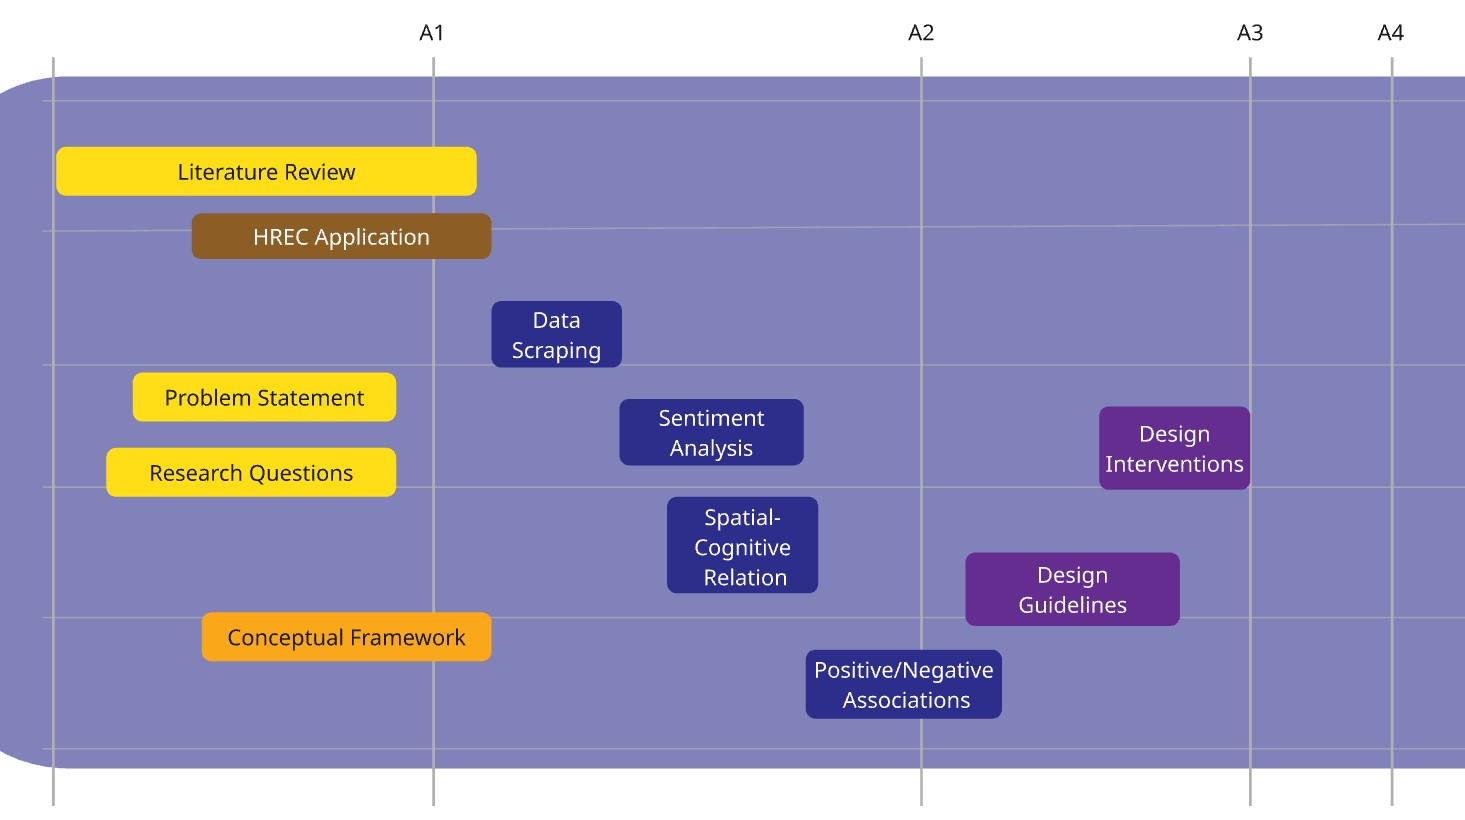
\includegraphics[keepaspectratio]{images/Timeframe.jpg}}

}

\caption{\emph{Figure 18. Project's timeline}}

\end{figure}%

\newpage{}

\section*{References}\label{references}
\addcontentsline{toc}{section}{References}

\phantomsection\label{refs}
\begin{CSLReferences}{1}{0}
\bibitem[\citeproctext]{ref-aleksandar}
Aleksandar, Asonja, · Evgeny, Panidi · Ayse, and Ozcan Buckley. n.d.
{``Sustainable Landscape Planning and Natural Resources Management IEREK
Interdisciplinary Series for Sustainable Development Integrating
Agriculture, Urban Systems, and Natural Resources a Pathway to
Sustainable Landscapes.''}

\bibitem[\citeproctext]{ref-arnstein2019}
Arnstein, Sherry R. 2019. {``A Ladder of Citizen Participation.''}
\emph{Journal of the American Planning Association} 85 (1): 24--34.
\url{https://doi.org/10.1080/01944363.2018.1559388}.

\bibitem[\citeproctext]{ref-currie2022}
Currie, Morgan, Jeremy Knox, and Callum Mcgregor. 2022. {``INTRODUCTION:
DATA JUSTICE AND THE RIGHT TO THE CITY.''}

\bibitem[\citeproctext]{ref-fathullah2018}
Fathullah, Afif, and Katharine S. Willis. 2018. {``Engaging the Senses:
The Potential of Emotional Data for Participation in Urban Planning.''}
\emph{Urban Science} 2 (4): 98.
\url{https://doi.org/10.3390/urbansci2040098}.

\bibitem[\citeproctext]{ref-habibi2016}
Habibi, Seyyed Mohsen, and Maryam Amiri. 2016. {``Right to the City: The
Existing City and the Desired City, What There Is and What Must Be {[}حق
به شهر: شهر موجود و شهر مطلوب آنچه هست و آنچه باید باشد{]}.''}
\emph{Journal of Iranian Human Studies} 5 (2): 9--30.

\bibitem[\citeproctext]{ref-harvey2003}
Harvey, David. 2003. {``The Right to the City.''} \emph{International
Journal of Urban and Regional Research} 27 (4): 939--41.
\url{https://doi.org/10.1111/j.0309-1317.2003.00492.x}.

\bibitem[\citeproctext]{ref-harvey2006}
---------. 2006. {``The Political Economy of Public Space.''} In, edited
by Setha M. Low and Neil Smith, 17--34. New York, NY: Routledge.
\url{https://doi.org/10.4324/9780203390306-2}.

\bibitem[\citeproctext]{ref-harvey2015}
---------. 2015. {``The Right to the City.''} In.

\bibitem[\citeproctext]{ref-haskins2007}
Haskins, Ekaterina. 2007. {``Between Archive and Participation: Public
Memory in a Digital Age.''} \emph{Rhetoric Society Quarterly} 37 (4):
401--22. \url{https://doi.org/10.1080/02773940601086794}.

\bibitem[\citeproctext]{ref-horelli2024}
Horelli, Liisa, and Sirkku Wallin. 2024. {``Civic Engagement in Urban
Planning and Development.''} \emph{Land} 13 (9): 1446.
\url{https://doi.org/10.3390/land13091446}.

\bibitem[\citeproctext]{ref-lefebvre1968}
Lefebvre, Henri. 1968. \emph{The Right to the City}.

\bibitem[\citeproctext]{ref-lynch1964}
Lynch, Kevin. 1964. \emph{THE IMAGE OF THE CITY}.

\bibitem[\citeproctext]{ref-macrotrends}
MacroTrends. n.d. {``Tehran, Iran Metro Area Population
(1950{\textendash}2026).''}

\bibitem[\citeproctext]{ref-martin2025}
Martin, Melissa. 2025. {``Public Participation in Urban Planning: How
Emotional Mapping Could Contribute to Building a Sense of Belonging.''}
In, edited by Asonja Aleksandar, Evgeny Panidi, and Ayse Ozcan Buckley,
77--85. Cham: Springer Nature Switzerland.
\url{https://link.springer.com/10.1007/978-3-031-81288-0_8}.

\bibitem[\citeproctext]{ref-mitchell2003}
Mitchell, Don. 2003. {``The End of Public Space? People's Park,
Definitions of the Public and Democracy.''}

\bibitem[\citeproctext]{ref-mohit2026}
Mohit. 2026. {``CITY THEATER.''}
\url{https://mohit.art/network/city-theatre/}.

\bibitem[\citeproctext]{ref-moroni2014}
Moroni, Stefano, and Francesco Chiodelli. 2014. {``Public Spaces,
Private Spaces, and the Right to the City.''} \emph{International
Journal of E-Planning Research} 3 (1): 51--65.
\url{https://doi.org/10.4018/ijepr.2014010105}.

\bibitem[\citeproctext]{ref-mueller2018}
Mueller, Johannes, Hangxin Lu, Artem Chirkin, Bernhard Klein, and
Gerhard Schmitt. 2018. {``Citizen Design Science: A Strategy for
Crowd-Creative Urban Design.''} \emph{Cities} 72 (February): 181--88.
\url{https://doi.org/10.1016/j.cities.2017.08.018}.

\bibitem[\citeproctext]{ref-paccoud2016}
Paccoud, Antoine. 2016. {``Planning Law, Power, and Practice: Haussmann
in Paris (1853{\textendash}1870).''} \emph{Planning Perspectives} 31
(3): 341--61. \url{https://doi.org/10.1080/02665433.2015.1089414}.

\bibitem[\citeproctext]{ref-shaw2017}
Shaw, Joe, and Mark Graham. 2017. {``An Informational Right to the City?
Code, Content, Control, and the Urbanization of Information.''}
\emph{Antipode} 49 (4): 907--27.
\url{https://doi.org/10.1111/anti.12312}.

\bibitem[\citeproctext]{ref-solnit2001}
Solnit, Rebecca. 2001. \emph{Wanderlust : A History of Walking}. {[}New
York, N.Y.{]}: Penguin Books, an imprint of Penguin Random House LLC.

\bibitem[\citeproctext]{ref-solnit2009}
---------. 2009. \emph{A Field Guide to Getting Lost}. Canongate Books.

\bibitem[\citeproctext]{ref-statcounter}
statcounter. n.d. {``Social Media Stats Islamic Republic of Iran.''}

\bibitem[\citeproctext]{ref-tedeschi2024}
Tedeschi, M. 2024. {``Datafication and Urban (in) Justice: Towards a
Digital Spatial Justice.''} \emph{Geography Compass}.
\url{https://doi.org/10.1111/gec3.12763}.

\bibitem[\citeproctext]{ref-wikipedia2026}
wikipedia. 2026. {``City Theater of Tehran.''}
\url{https://en.wikipedia.org/wiki/City_Theater_of_Tehran}.

\bibitem[\citeproctext]{ref-williamson2020}
Williamson, Wayne, and Kristian Ruming. 2020. {``Can Social Media
Support Large Scale Public Participation in Urban Planning? The Case of
the {\#}MySydney Digital Engagement Campaign.''} \emph{International
Planning Studies} 25 (4): 355--71.
\url{https://doi.org/10.1080/13563475.2019.1626221}.

\end{CSLReferences}




\end{document}
